\documentclass{beamer}
\usetheme{default}

\usepackage{caption}
\usepackage{subcaption}

% width of figures
\newcommand\w{0.32}

\title{1m structure method development}
\author{T.\ Northey}
\date{4 Oct 2022 group meeting}
\begin{document}
\begin{frame}[plain]
    \maketitle
\end{frame}

\begin{frame}
	% start the columns environment    
	\begin{columns} 
		% Column 1
		\begin{column}{.4\textwidth}
			\begin{figure}[H]
				\centering
				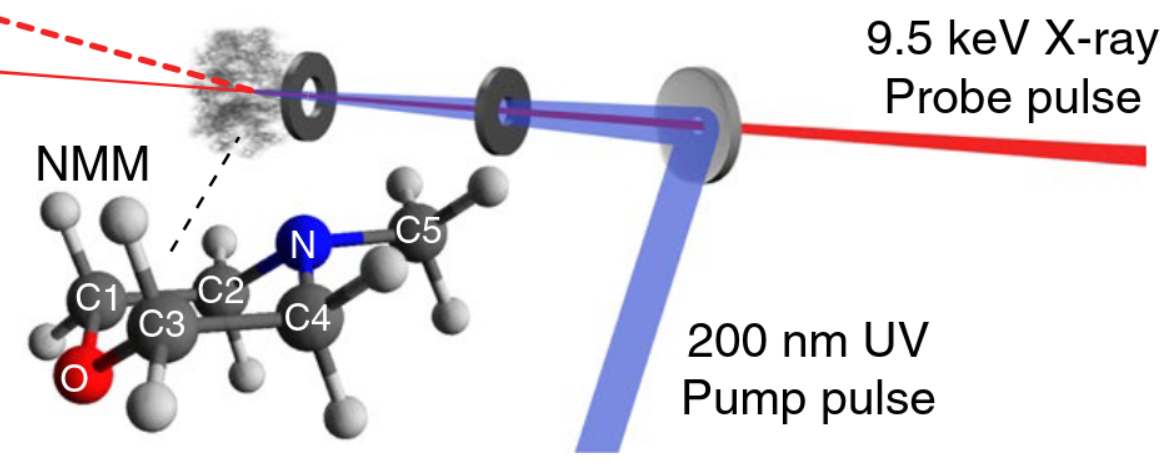
\includegraphics[width=\textwidth]{nmm_geometry.png}
				\caption{NMM geometry, and experimental setup.}
				\label{fig:nmm-geom}
			\end{figure}
			\begin{itemize}
				\item 107 surface hopping trajectories (1000 fs), $\sim$$10^6$ molecular geometries 
			\end{itemize}
			{\tiny B.\ Stankus, et al.\ Nature Chem.\ 11.8 (2019):\ 716-721.}
		\end{column}
		% Column 2    
		\begin{column}{.6\textwidth}
			\begin{figure}[H]
				\centering
				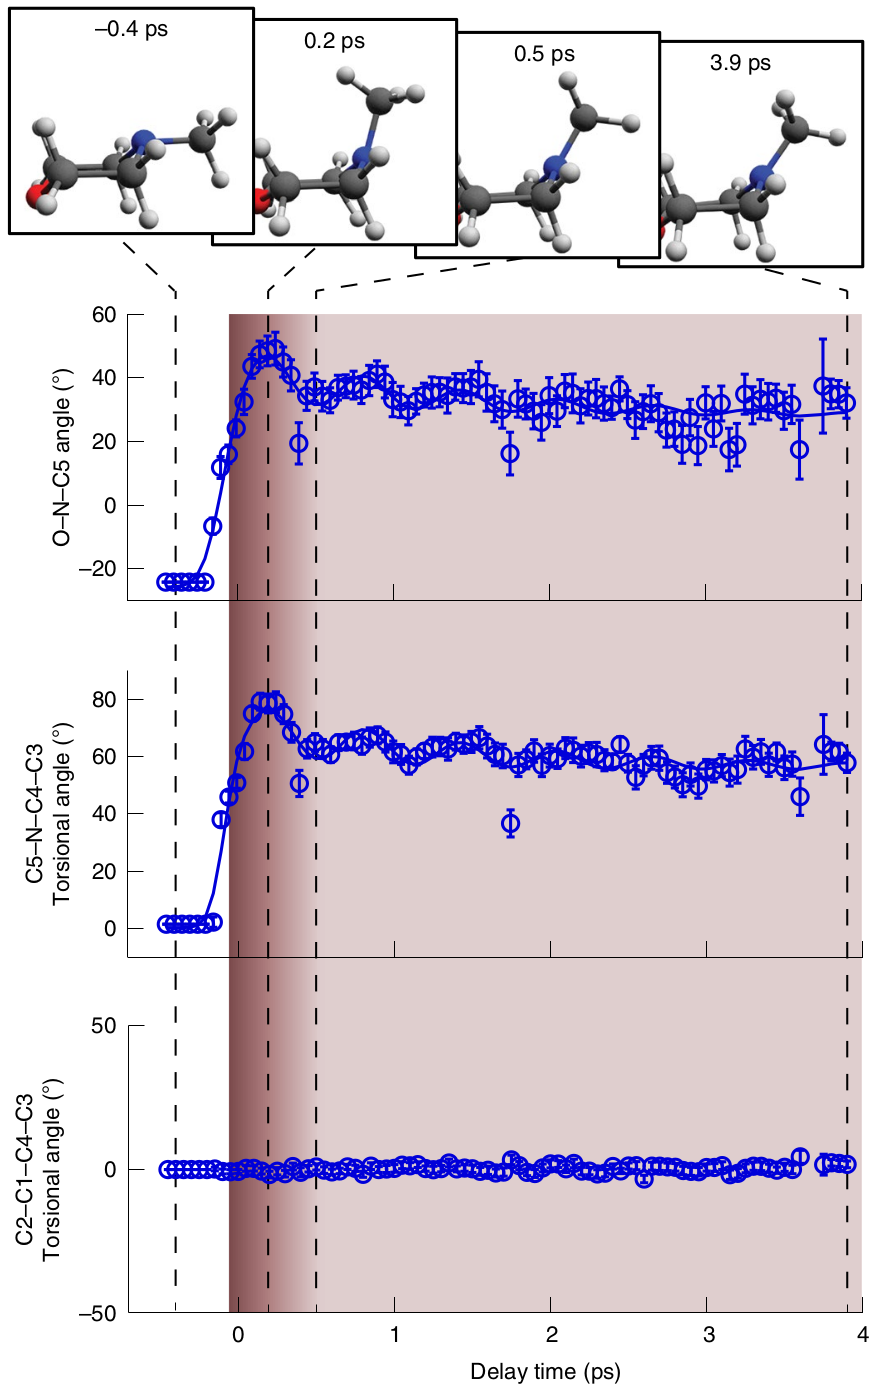
\includegraphics[width=0.7\textwidth]{stankus_angle_plots.png}
				\caption{Time-dependent angle plots
					following Rydberg excitation.}
				\label{fig:nmm-geom}
			\end{figure}
		\end{column}%
		
	\end{columns}
\end{frame}

%\begin{frame}{Defining structure pool parameters}
%\begin{center}
%	{\huge$\mu$}\qquad\qquad{\huge$\sigma_i$}\\
%	\vspace{2cm}
%	{\huge$\rho$}
%\end{center}
%\end{frame}


%\begin{frame}{Defining structure pool parameters}
%		\begin{center}
%	{\huge$\mu=0$, e.g.\ $\textbf{R}_0$}
%		\end{center}
%	
%	[picture of potential energy curve along a bond-distance, + bell curve vibrational distribution]
%	
%	[and picture of $\mu\neq 0$ situation, shifted bell curve]
%\end{frame}

%\begin{frame}{Defining structure pool parameters}
%		\begin{center}
%	$\sigma=\begin{pmatrix}
%	0.4 \\
%	0.2\\
%	0.2\\
%	\vdots\\
%	0.2
%	\end{pmatrix}
%	$ \AA
%		\end{center}
%	
%	\begin{itemize}
%		\item some displacements more important than others
%		\item some could be irrelevant $\sigma_i = 0$ (i.e.\ don't displace at all)
%	\end{itemize}
%
%\end{frame}

%\begin{frame}{Defining structure pool parameters}
%		\begin{center}
%	\qquad\qquad\qquad\ \ \ {\huge$\rho\propto\textrm{accuracy / resolution}$}\\
%		\vspace{2mm}
%	{\huge$\propto N$}\\
%		\vspace{2mm}
%	\quad\ \ {\huge$\propto 1/\sigma_i$}\\
%	%\qquad\qquad\qquad\ \ {\huge$\propto 1/n_{\textrm{modes}}$}\\
%		\end{center}
%\end{frame}



\begin{frame}
	% start the columns environment    
	\begin{columns} 
		% Column 1
		\begin{column}{.4\textwidth}
			\begin{figure}[H]
				\centering
				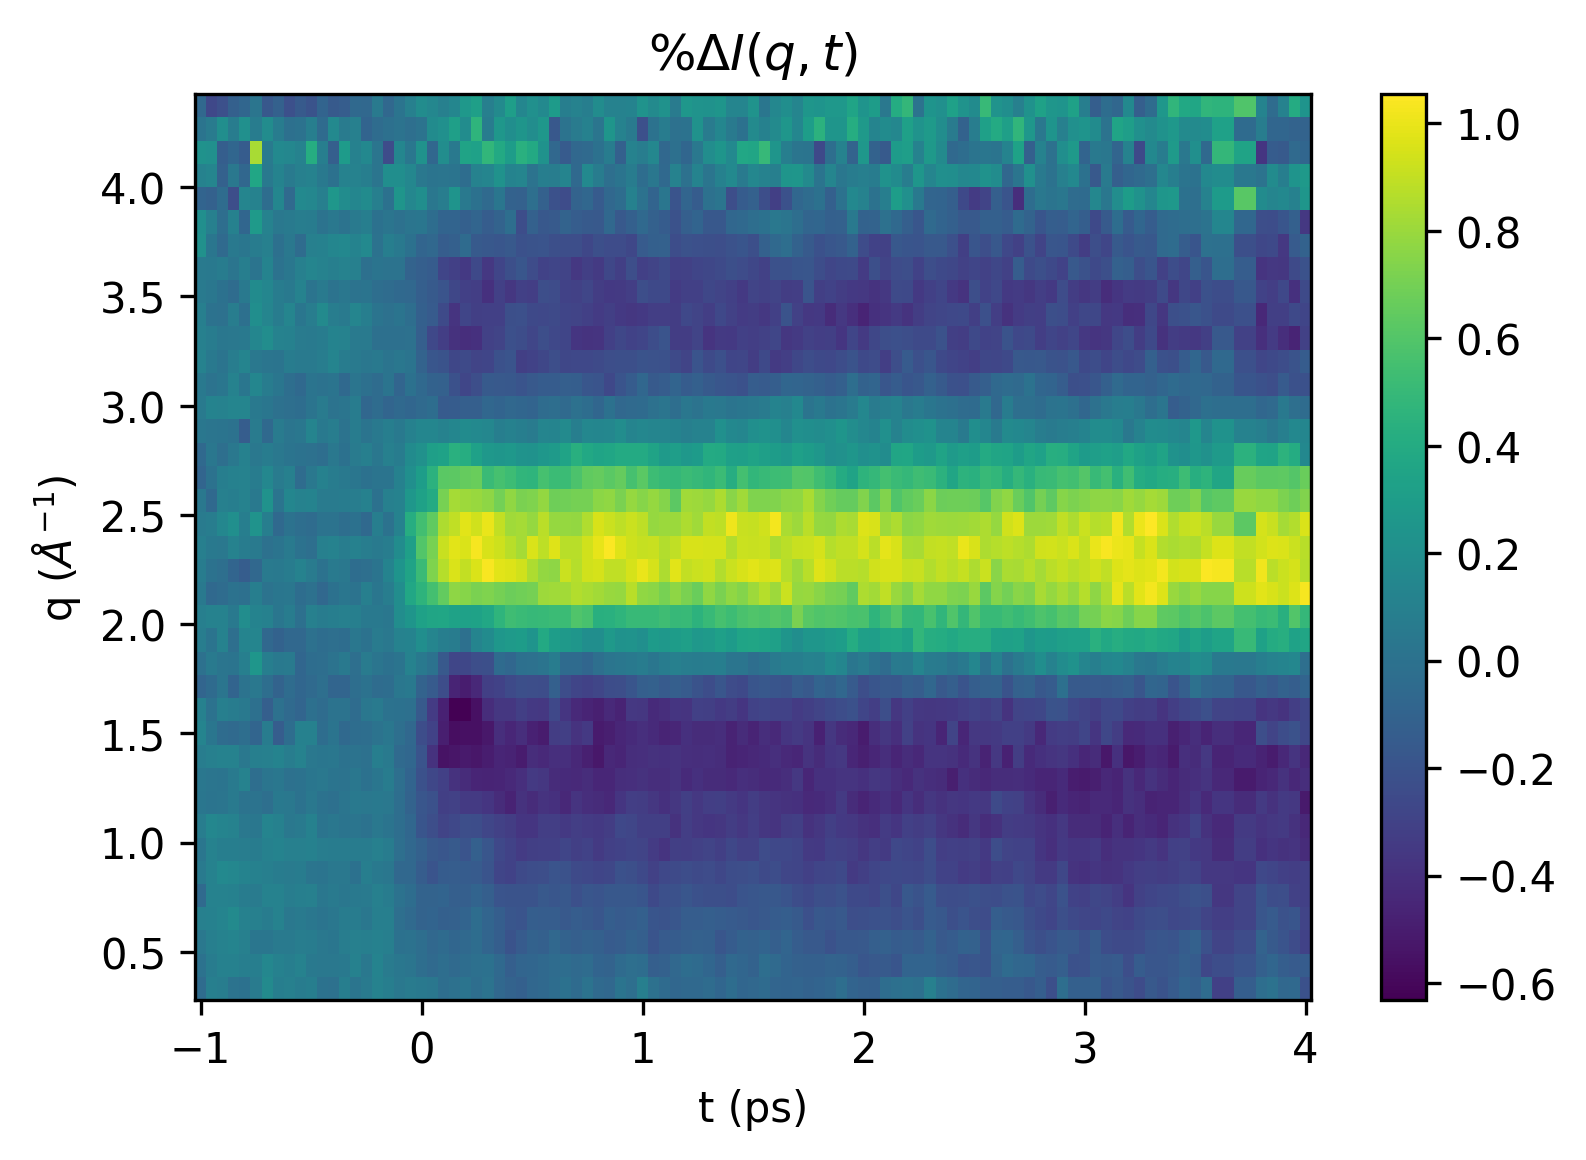
\includegraphics[width=\textwidth]{NMM_exp_2Dplot.png}
				\caption{Time-resolved x-ray scattering percent difference signal for NMM.}
				\label{fig:nmm-2dplot}
			\end{figure}
			\vspace{-5mm}
			\begin{itemize}
				\item $q = [0.33, 4.37] $ \AA$^{-1}$, (with 39 $q$-bins)
				\item Excitation percentage, 5.7\%
				\item Maximum signal difference $\simeq 1\%$
			\end{itemize}
		\end{column}
		% Column 2    
		\begin{column}{.6\textwidth}
			\begin{figure}[H]
				\centering
				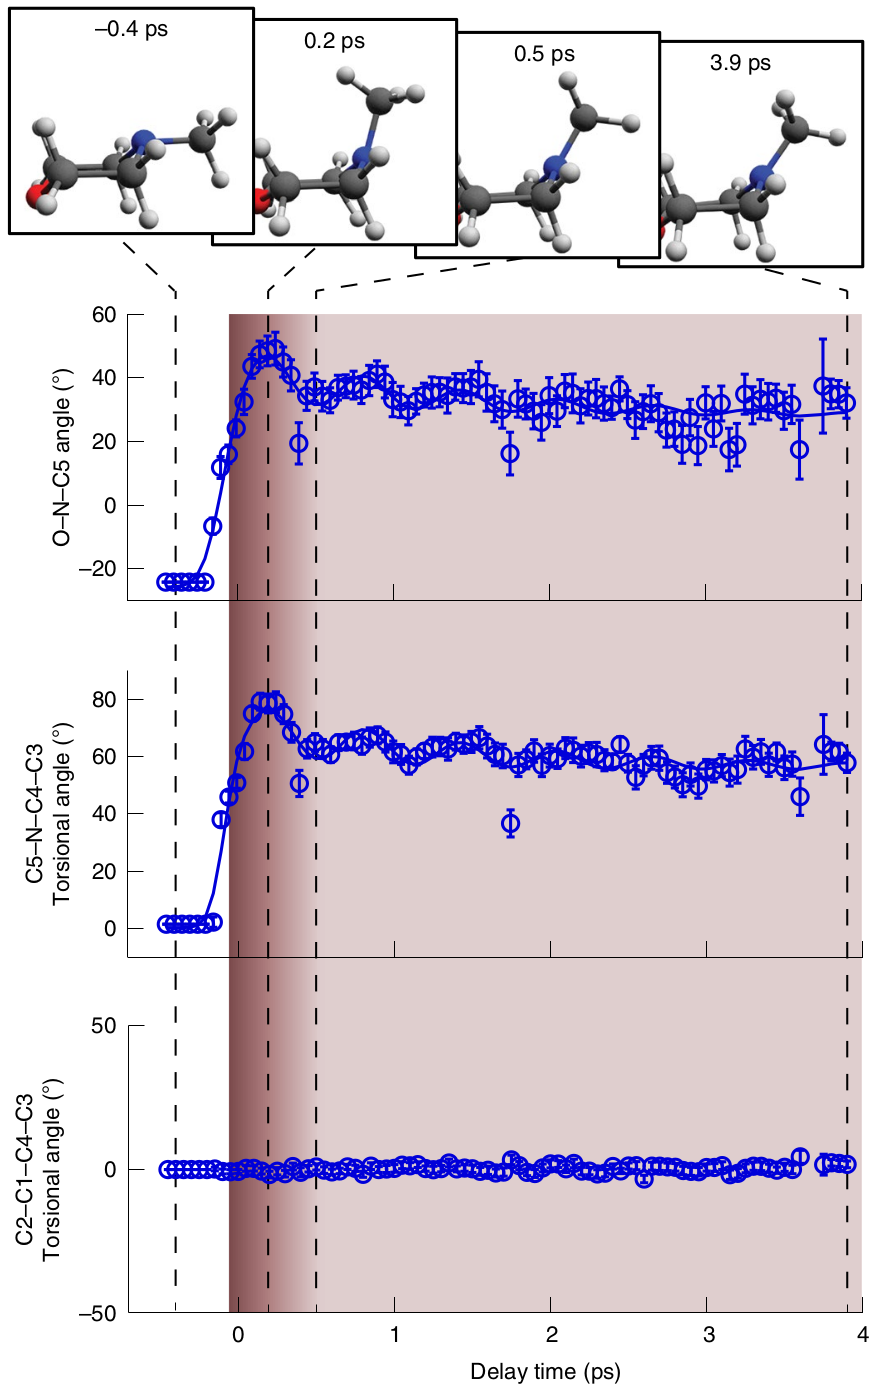
\includegraphics[width=0.7\textwidth]{stankus_angle_plots.png}
				\caption{Time-dependent angle plots
					following Rydberg excitation.}
				\label{fig:nmm-geom}
			\end{figure}
		\end{column}%
	\end{columns}
\end{frame}

\begin{frame}{Motivation}
	% start the columns environment    
$\bullet$ The 1m structure method is a sampling method to fit molecular structures to an experimental signal (i.e.\ time-resolved x-ray scattering), it should find the most likely trajectory
	\begin{columns} 
		% Column 1
		\begin{column}{.5\textwidth}
			\begin{itemize}
				\item Previous work (Yong et al.\ Faraday Disc.\ 2021) showed that different methods of generating the structure pool work (e.g.\ Wigner, MC, MD) as long as you sample the relevant molecular conformational space 
				\item They show that clamping the C-H bonds is an improvement in terms of the structure pool			
			\end{itemize}
		\end{column}
		% Column 2    
		\begin{column}{.5\textwidth}
			\begin{itemize}
				\item They used a 1000 K Wigner distribution to achieve enough vibrational amplitude for relevant geometries to be included, for the N-methylmorpholine photochemical reaction (pumped at 200 nm)
			\end{itemize}
		\begin{figure}
			\centering
			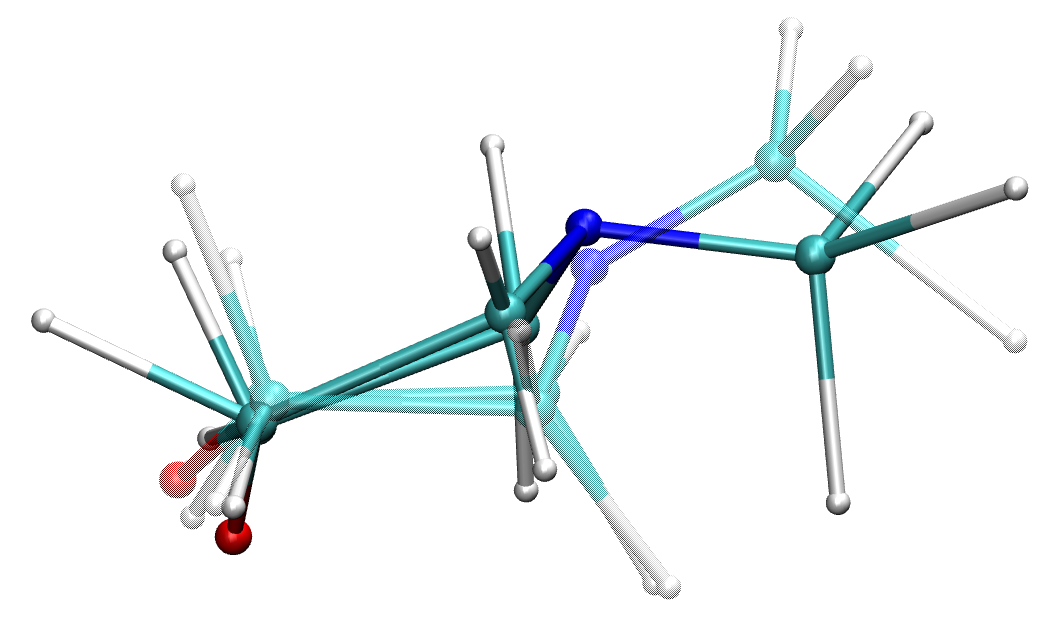
\includegraphics[width=0.5\textwidth]{allmodes_1m_2m_frame10_comparison.png}
		\end{figure}
		\end{column}%
	\end{columns}
\end{frame}

\begin{frame}{Method development}
	% start the columns environment  
				Goal: Improve million structure method; ideally lower $N$ needed, looking towards \textit{ab initio} calculations on each structure (e.g.\ to model photoelectron spectra, or if \textit{ab initio} x-ray calculations are required for certain systems)  
	\begin{columns} 
		% Column 1
		\begin{column}{.6\textwidth}
			\begin{enumerate}
				\item `modified' Wigner distribution; sample along the fully descriptive $3N-6$ normal modes (avoid $\frac{1}{2}N(N-1)$ scaling)
				\item Clamp all non-relevant motions (not only C-H bonds)
				\item ``Heat" most relevant motions	
			\end{enumerate}
		\end{column}
		% Column 2    
		\begin{column}{.4\textwidth}
			\begin{itemize}
				\item Try to model the NMM system, compare to Yong (2019)
			\end{itemize}
		\begin{figure}
			\centering
			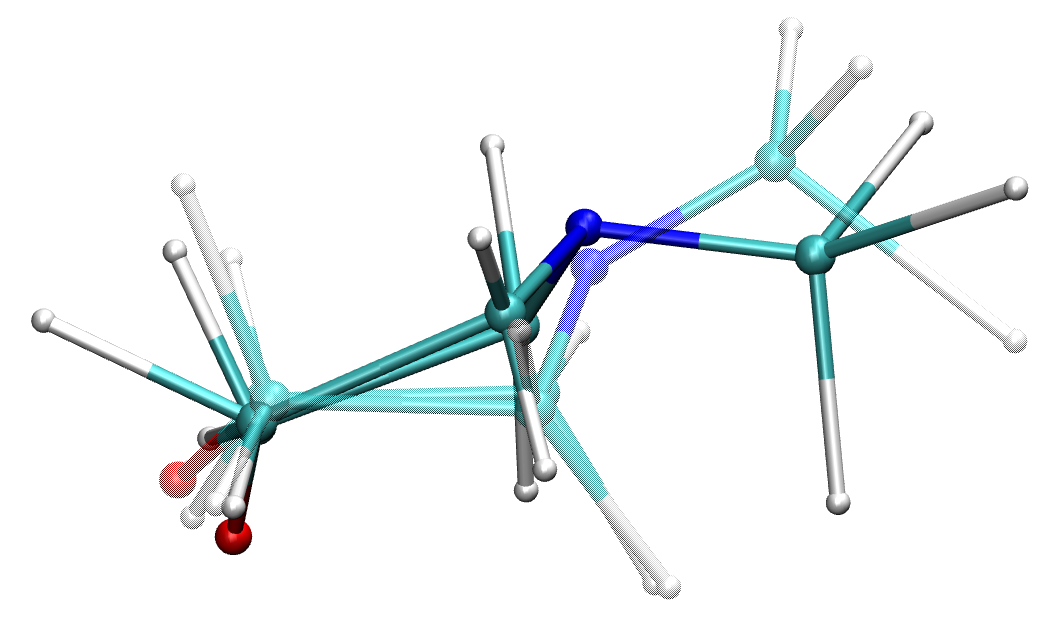
\includegraphics[width=0.5\textwidth]{allmodes_1m_2m_frame10_comparison.png}
		\end{figure}
		\end{column}%
	\end{columns}
\end{frame}

\begin{frame}{A sampling problem}
	\begin{columns}
		\begin{column}{0.5\textwidth}
			\begin{figure}
				\centering
				\begin{subfigure}[b]{\textwidth}
					\centering
					% left, bottom, right, top
					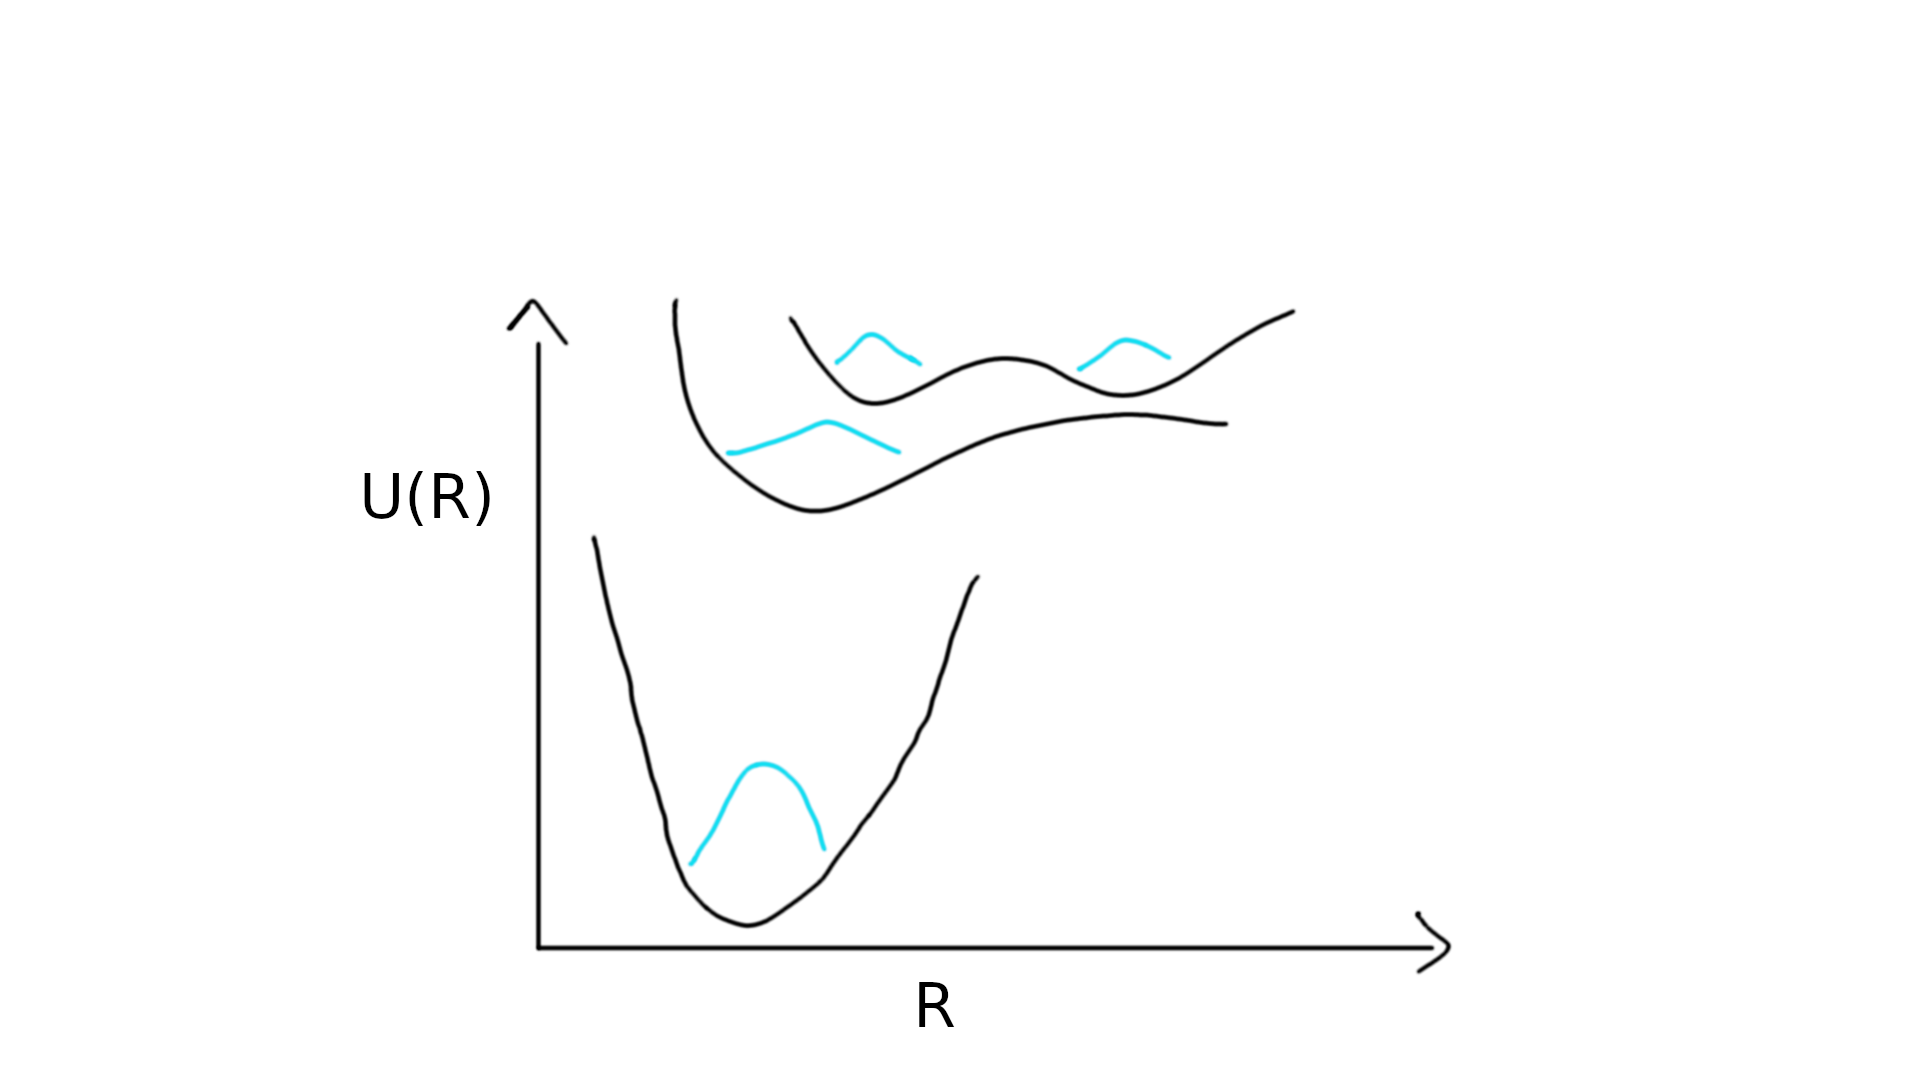
\includegraphics[width=\textwidth, trim= 80 10 58 70, clip]{multi_wigner.png}
					\caption{Option 1.}
					\label{fig:ur}
				\end{subfigure}
				\begin{subfigure}[b]{\textwidth}
					\centering
					% left, bottom, right, top
					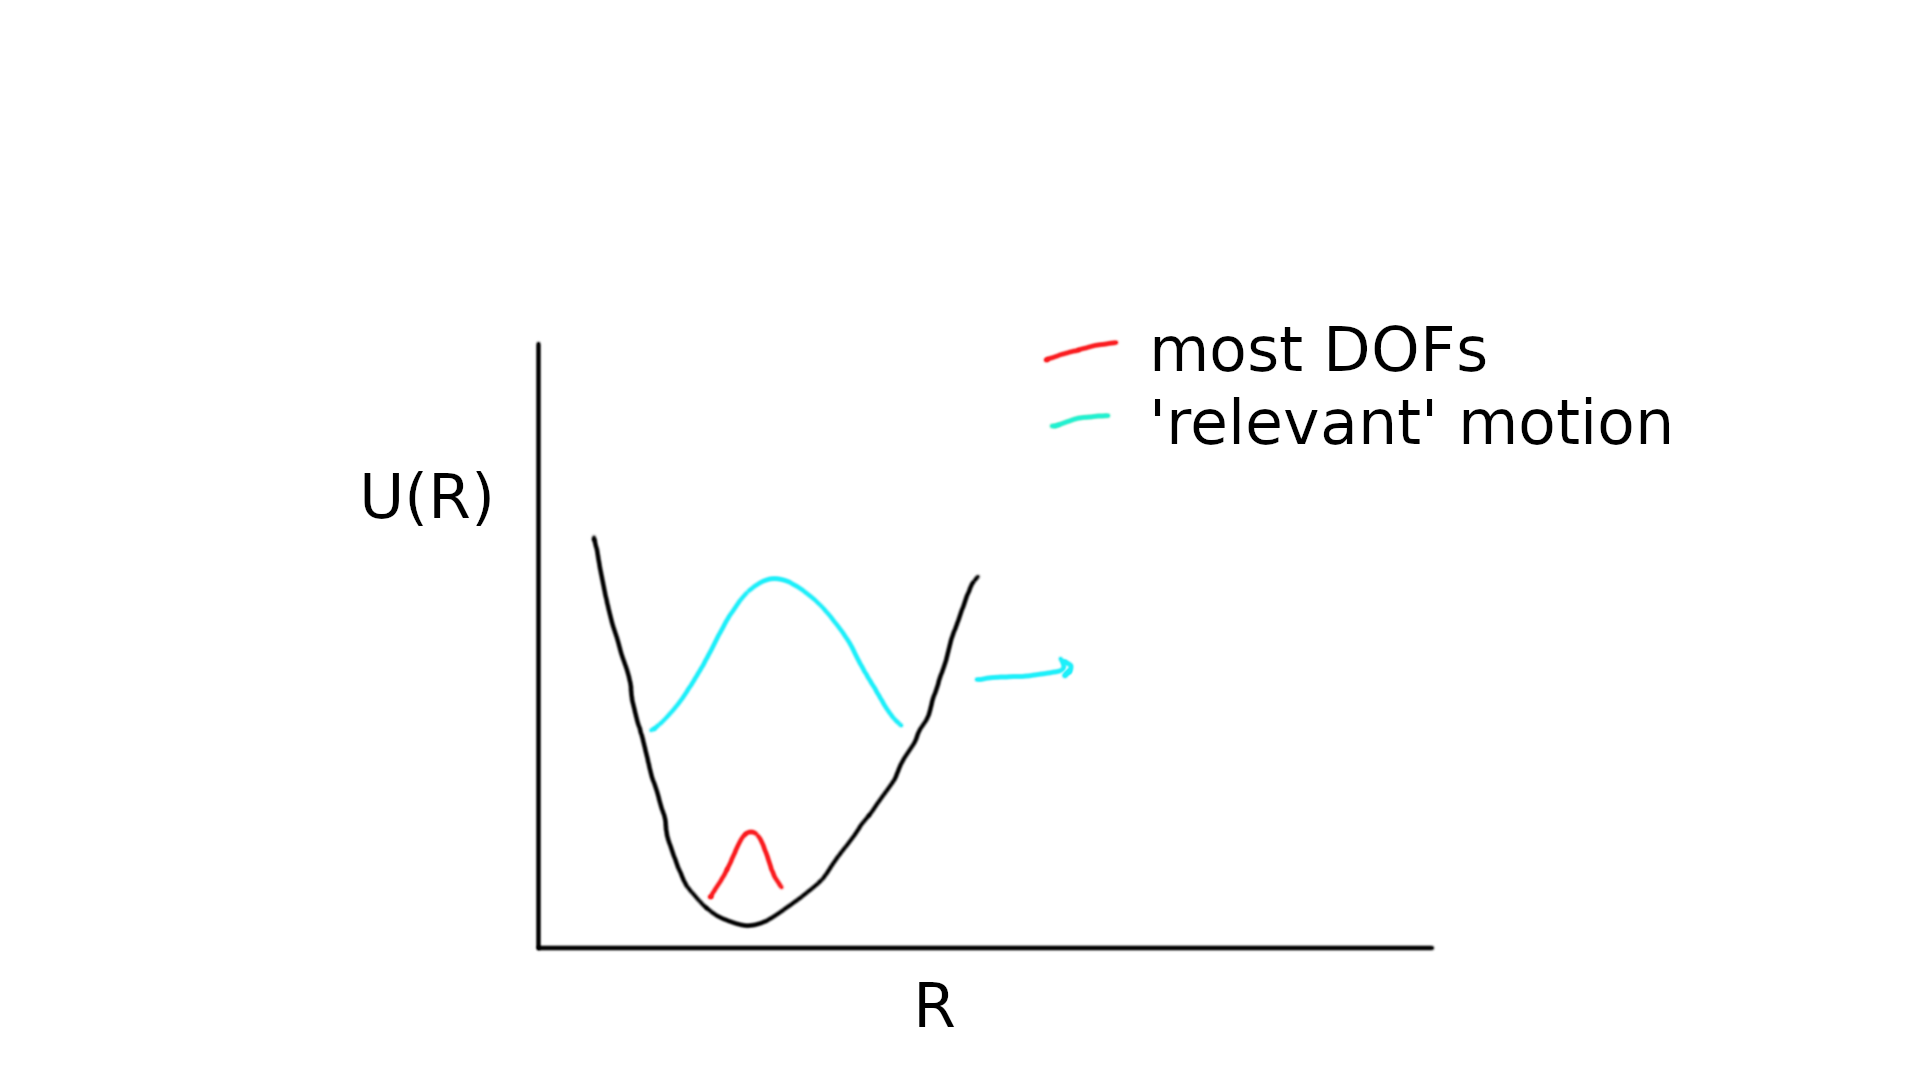
\includegraphics[width=\textwidth, trim= 80 10 58 70, clip]{modified_wigner.png}
					\caption{Option 2.}
					\label{fig:ur2}
				\end{subfigure}
			\end{figure}
		\end{column}
		\begin{column}{0.5\textwidth}
			\begin{itemize}
				\item Option 1: multiple structure pools at different excited states
				\begin{itemize}
					\item can sample far from $\textbf{R}_0$
				\end{itemize}
				\item Option 2: Sample a wider distribution around $\textbf{R}_0$
				\begin{itemize}
					\item simpler, avoids excited state calculations. 
					\item more like a black box solution (better for automation, code)
					\item still can sample away from the starting point to a certain extent (increase width of relevant motion)
				\end{itemize}
			\end{itemize}
		\end{column}	
	\end{columns}
\end{frame}

\begin{frame}{Method description}
	\begin{itemize}
	\item Geometry optimisation, frequency calculation
	\item	The sampling equation for generating the displaced molecular coordinates is,
	\[
	\textbf{R} = \textbf{R}_0 + \sum_i^{\textrm{modes}} a_i\hat{d}_i
	\]
	with starting geometry $\textbf{R}_0$, and displacement unit vectors $\hat{d}_i$ for each normal mode (from frequency calculation).  The factors $a_i$ are randomly generated within a Gaussian distribution centered at $\mu=0$, and chosen standard deviation, $\sigma_i \propto T$.

	\item Loop over the entire pool comparing the IAM percent difference (wrt $\textbf{R}_0$) to experiment; the structures with the lowest $\chi^2=(\textrm{theory}-\textrm{experiment})^2$ at each $t$ gives the best fit molecular trajectory.	
	\end{itemize}
\end{frame}

\begin{frame}{Distance histogram examples}
	\begin{figure}
		\centering
		\begin{subfigure}[b]{0.45\textwidth}
			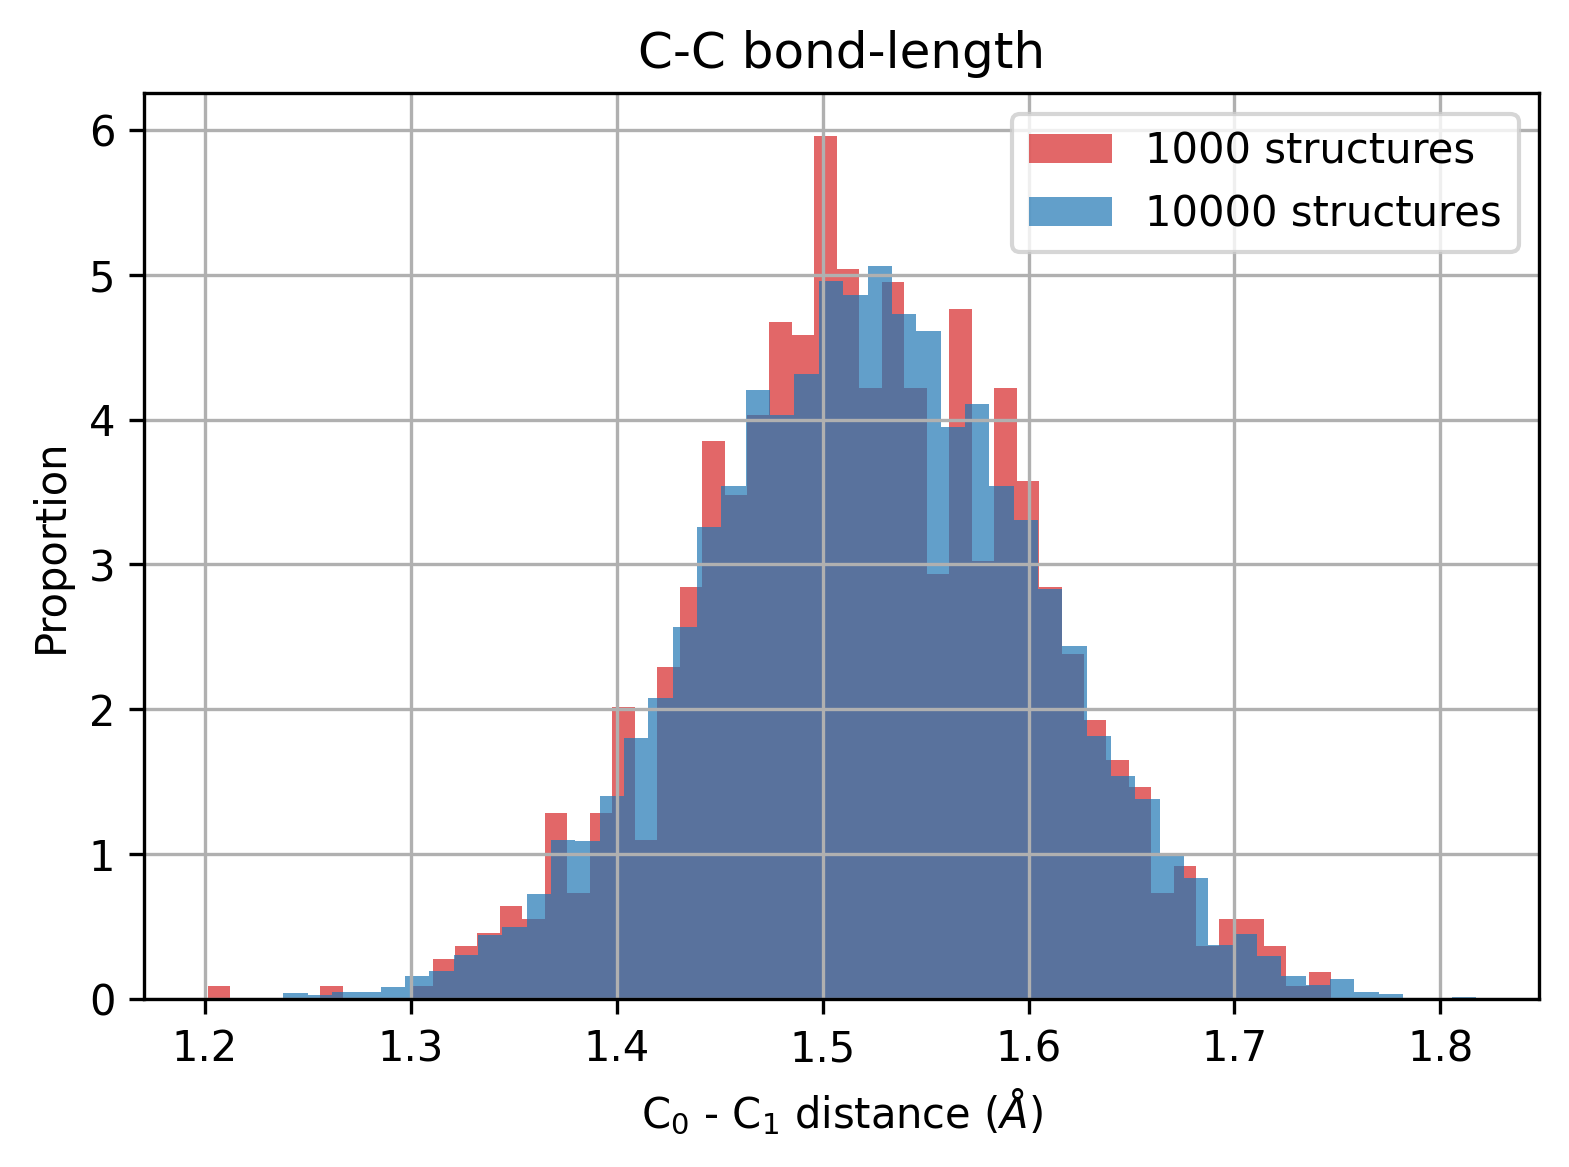
\includegraphics[width=\textwidth]{../notebooks/C_C_bond_length_hist.png}
		\end{subfigure}
		\begin{subfigure}[b]{0.45\textwidth}
			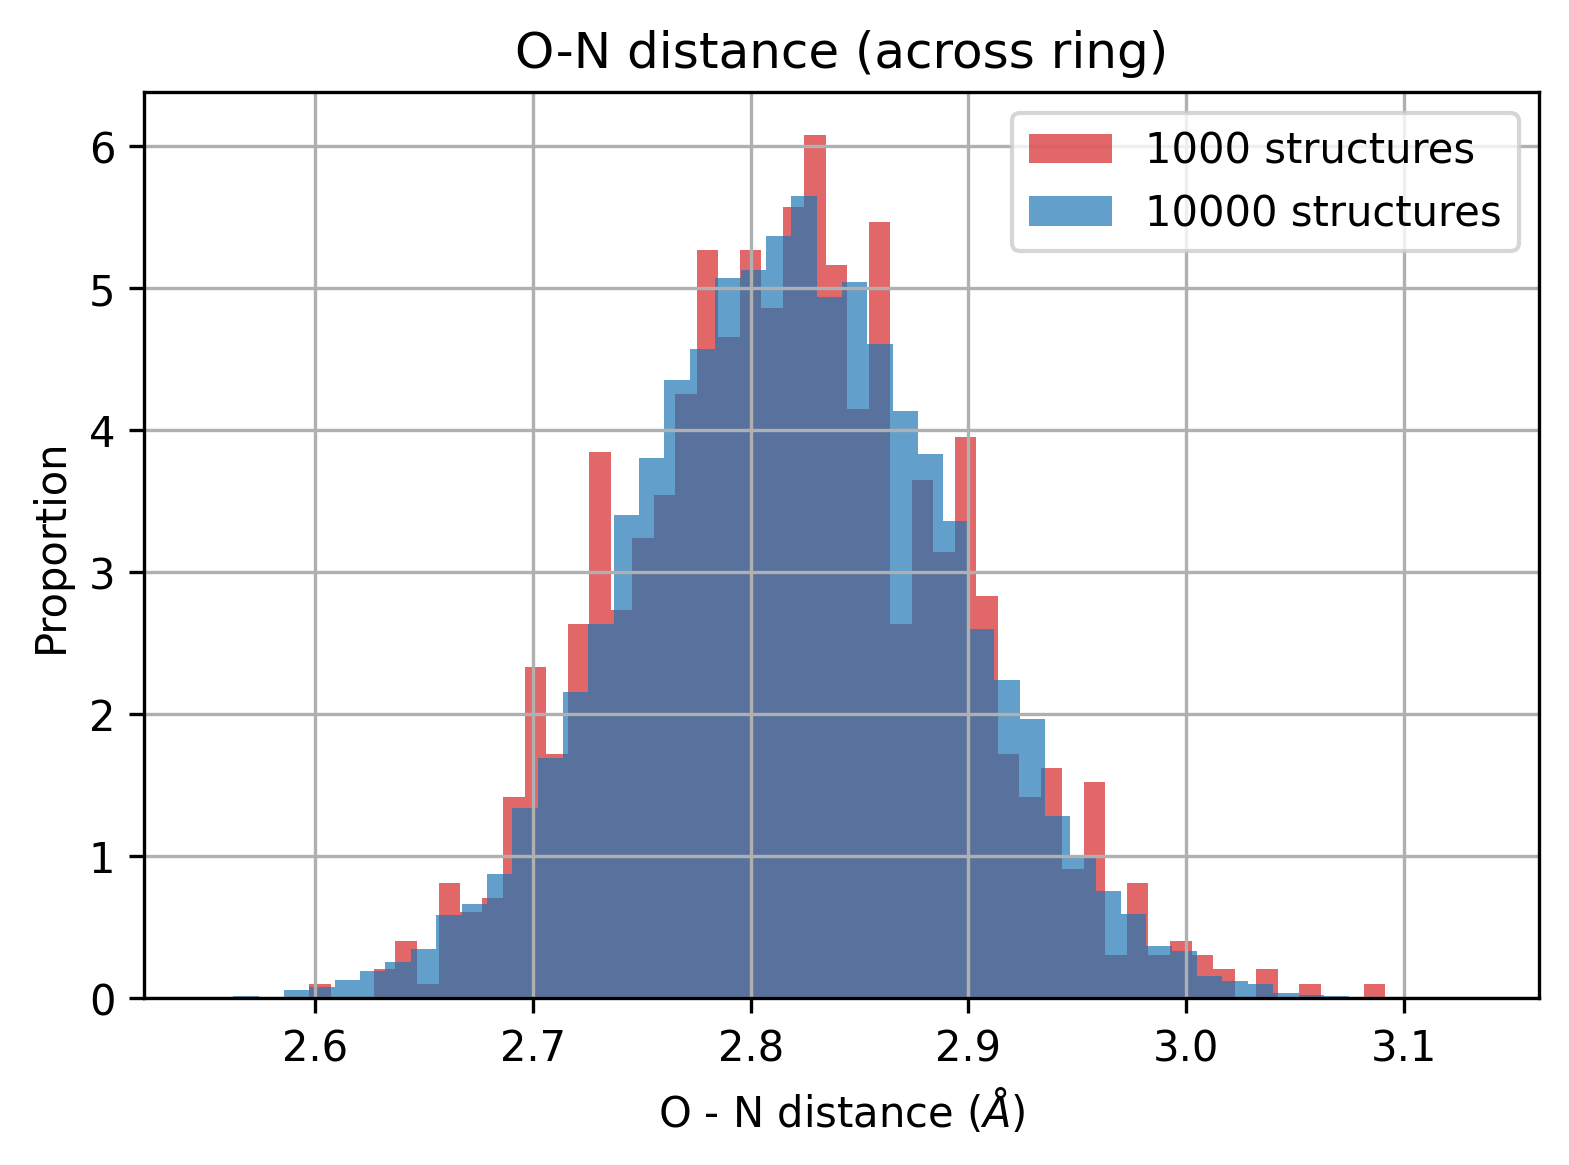
\includegraphics[width=\textwidth]{../notebooks/O_N_bond_length_hist.png}
		\end{subfigure}
	\end{figure}
	\begin{itemize}
		\item All geometry coordinates fall into a bell curve distribution centered at the molecule's starting position
		\item Therefore the pool is (reasonably) realistic 
	\end{itemize}
\end{frame}

%\begin{frame}{NMM previous work}
%	\begin{figure}[H]
%	\centering
%		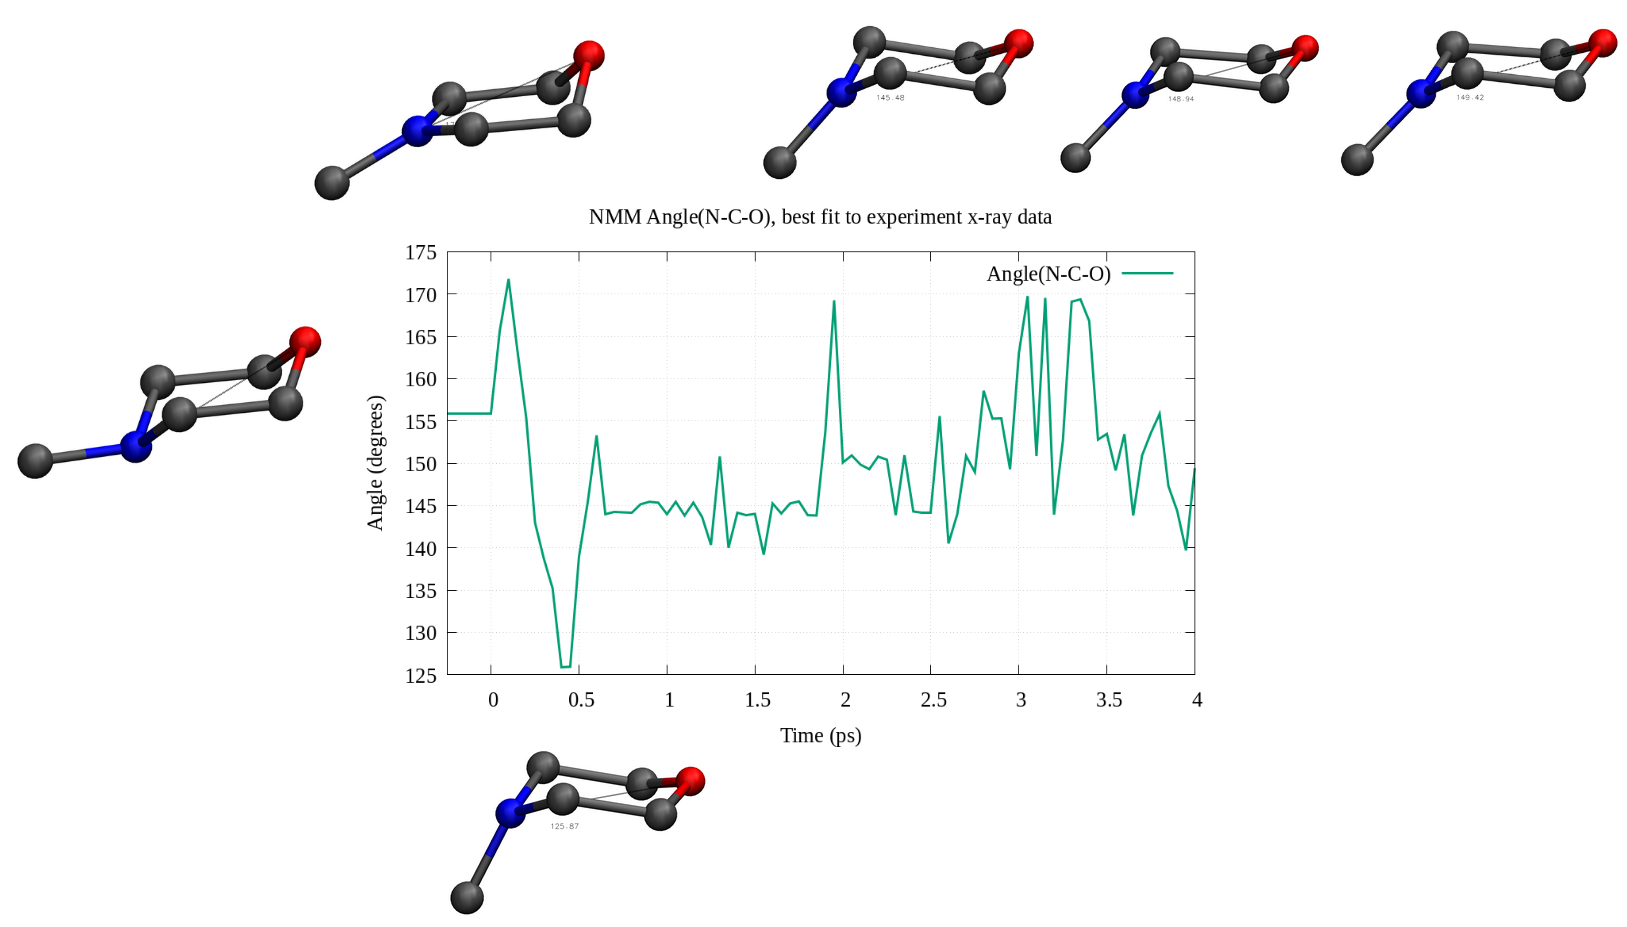
\includegraphics[width=\textwidth]{geomovie_ppt_slide.png}
%		\caption{N-C-O angle, best fit to experiment x-ray data.}
%		\label{fig:geomovie-ppt-slide}
%	\end{figure}
%
%\end{frame}

\begin{frame}{NMM normal modes}
	\newcommand{\x}{0.18}
	\begin{figure}
		\centering
		\begin{subfigure}{\x\textwidth}
			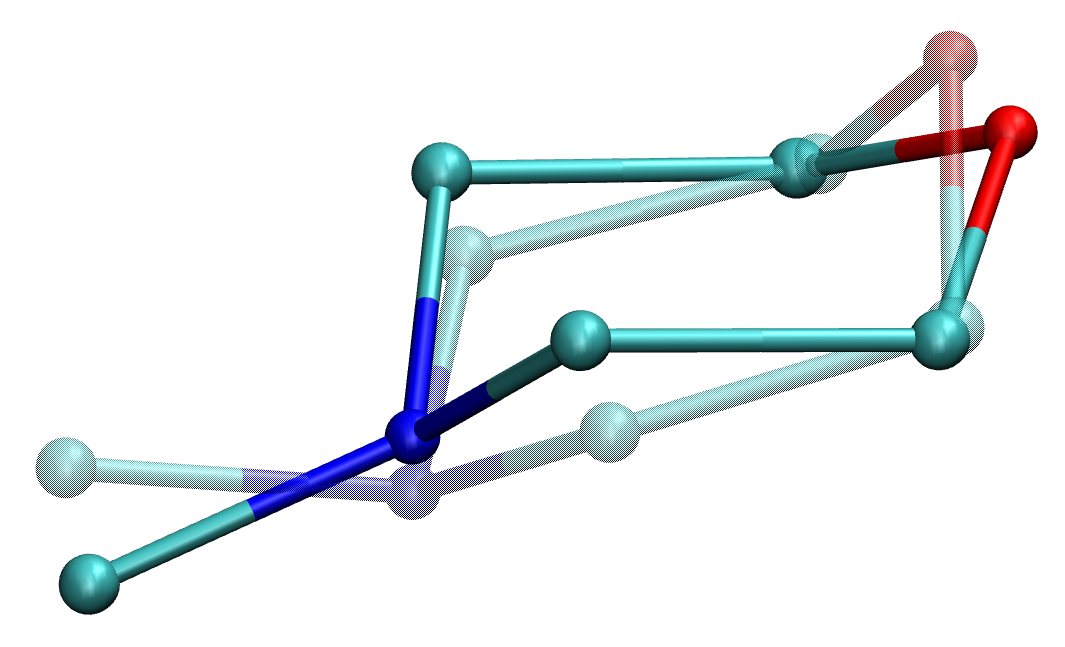
\includegraphics[width=\textwidth]{mode0_ot.png}
			\caption{mode 0: ``methyl swing"}
		\end{subfigure}
		\begin{subfigure}{\x\textwidth}
			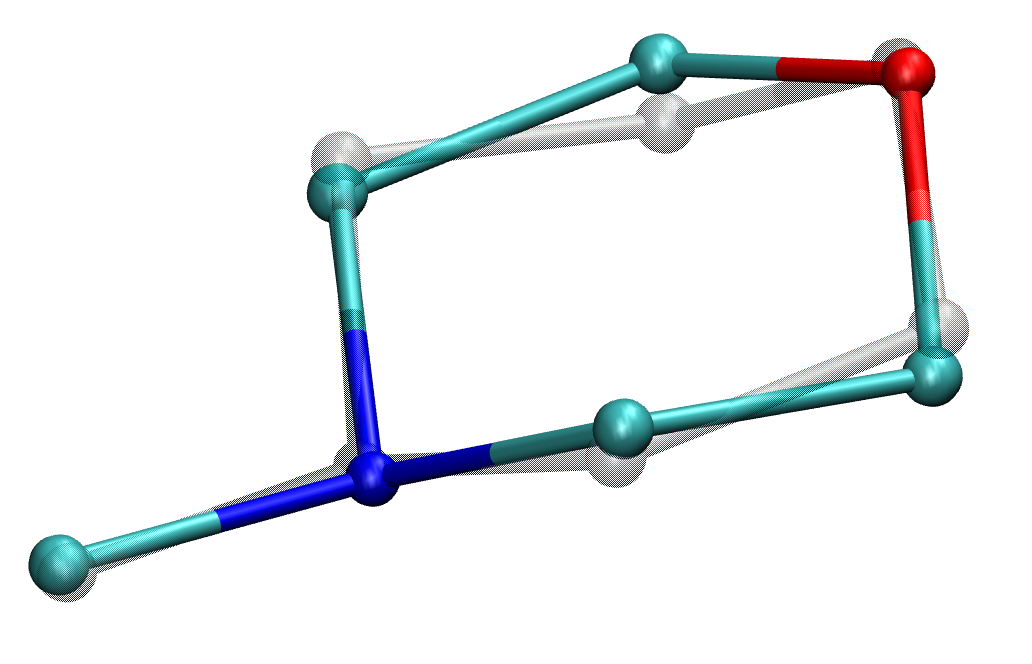
\includegraphics[width=\textwidth]{mode1_ot.png}
			\caption{mode 1: ``ring-twist"}
		\end{subfigure}
		\begin{subfigure}{\x\textwidth}
			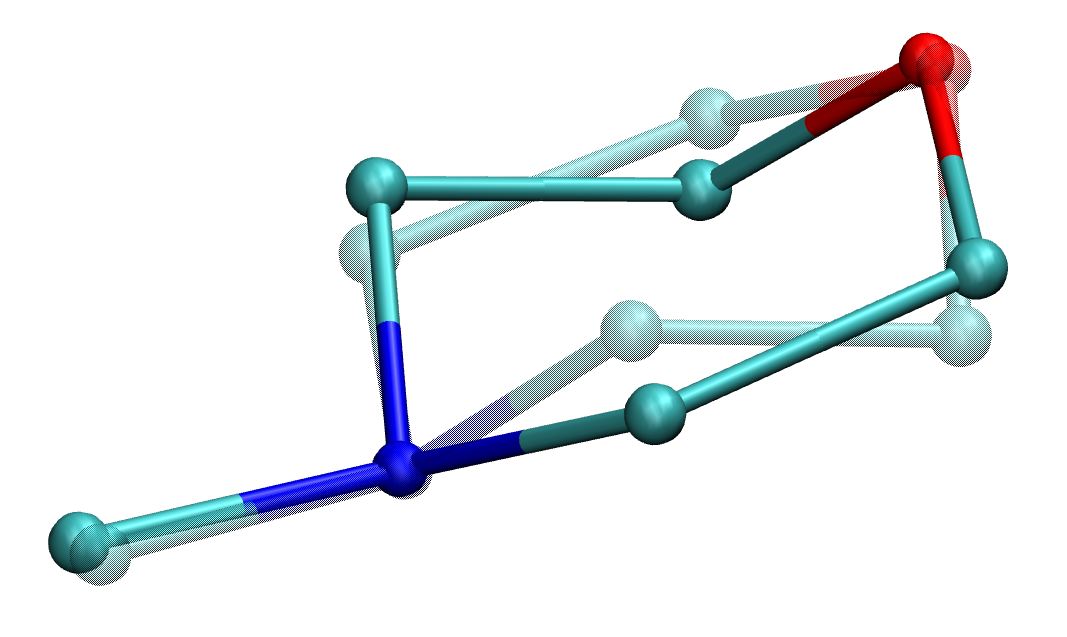
\includegraphics[width=\textwidth]{mode2_ot.png}
			\caption{mode 2: ``ring twist"}
		\end{subfigure}	
		\begin{subfigure}{\x\textwidth}
			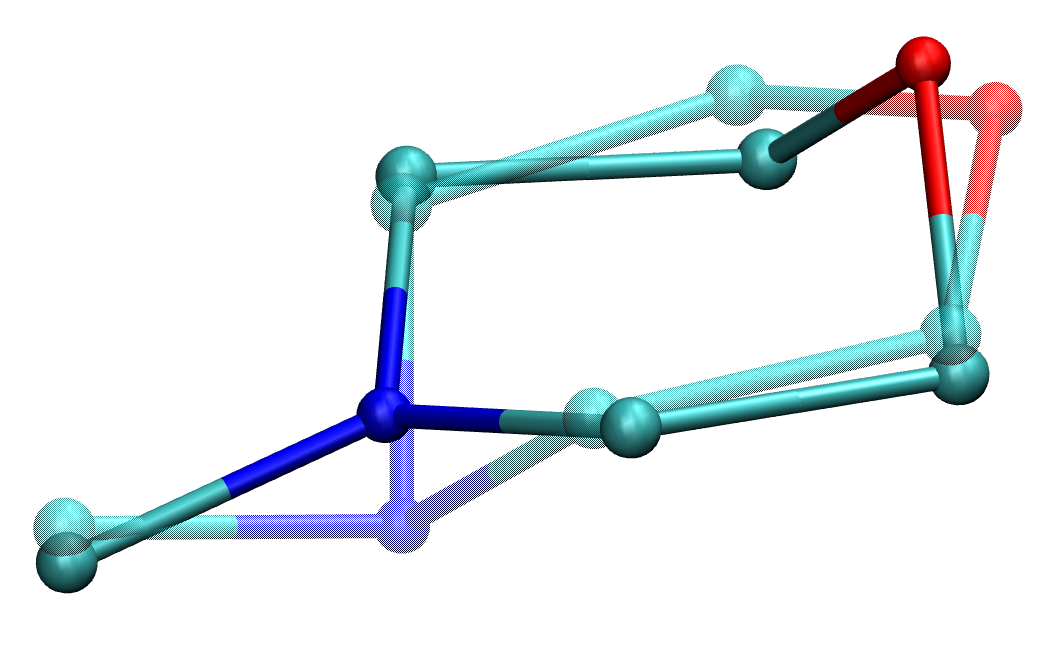
\includegraphics[width=\textwidth]{mode3_ot.png}
			\caption{mode 3: ``methyl swing"}
		\end{subfigure}
		\begin{subfigure}{\x\textwidth}
			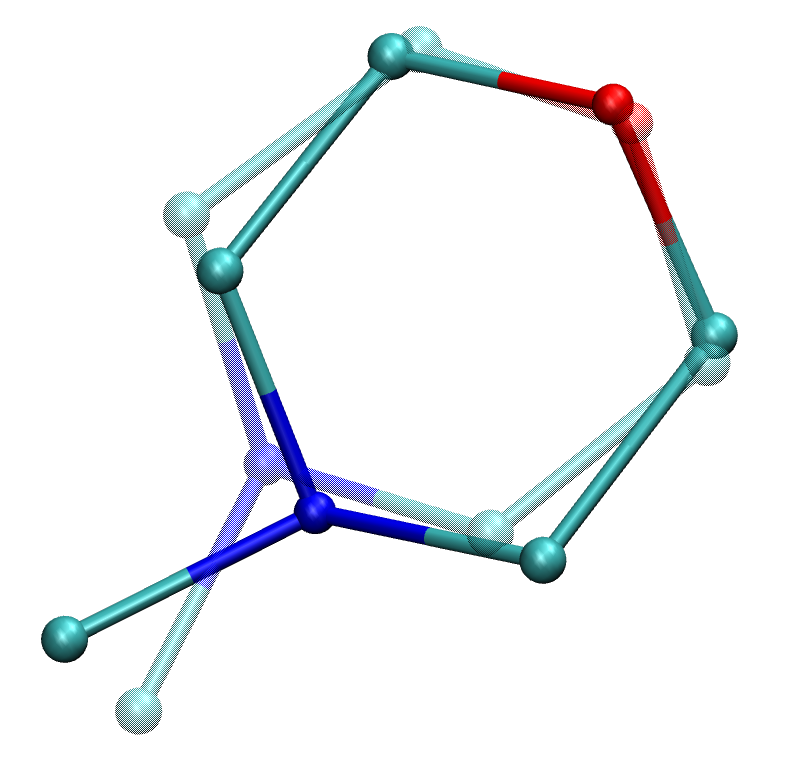
\includegraphics[width=\textwidth]{mode4_ot.png}
			\caption{mode 4: ``methyl side-to-side"}
		\end{subfigure}
		\begin{subfigure}{\x\textwidth}
			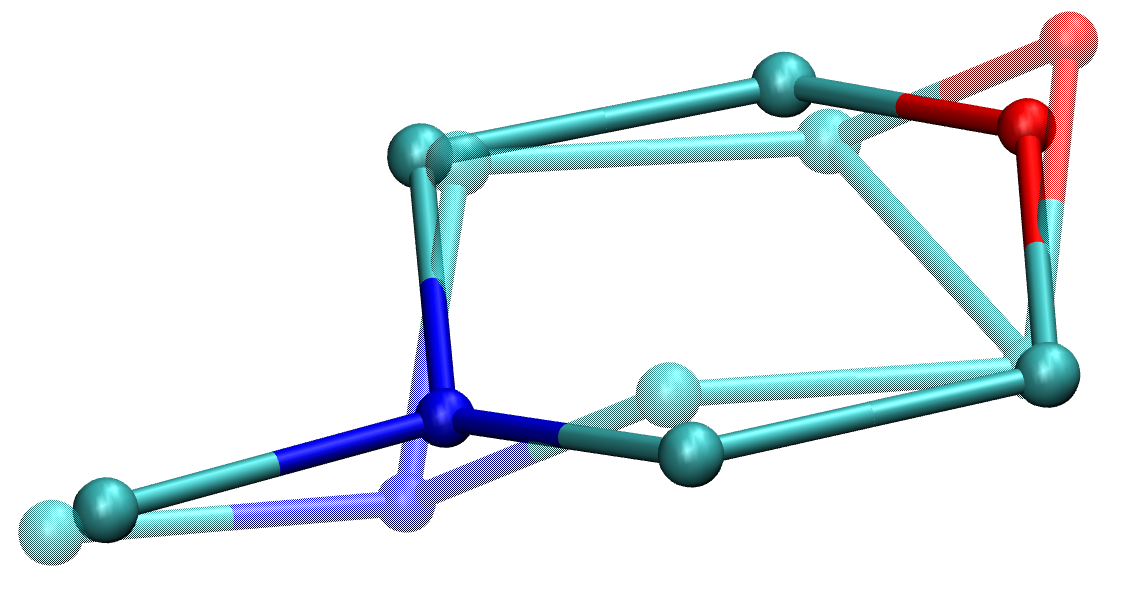
\includegraphics[width=\textwidth]{mode5_ot.png}
			\caption{mode 5: ``ring elongation"}
		\end{subfigure}				
		\begin{subfigure}{\x\textwidth}
			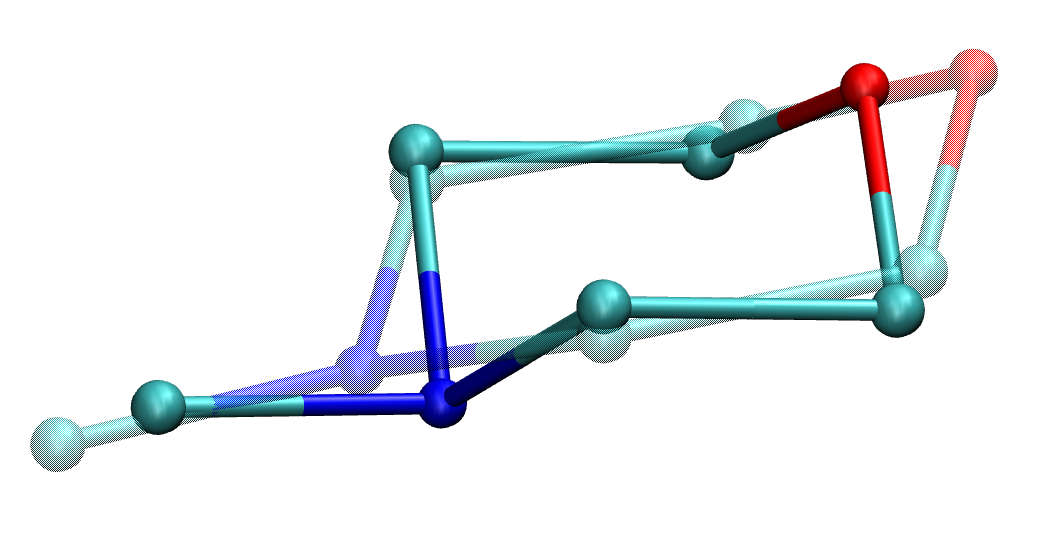
\includegraphics[width=\textwidth]{mode6_ot.png}
			\caption{mode 6: ``oxygen-methyl elongation"}
		\end{subfigure}
		\begin{subfigure}{\x\textwidth}
			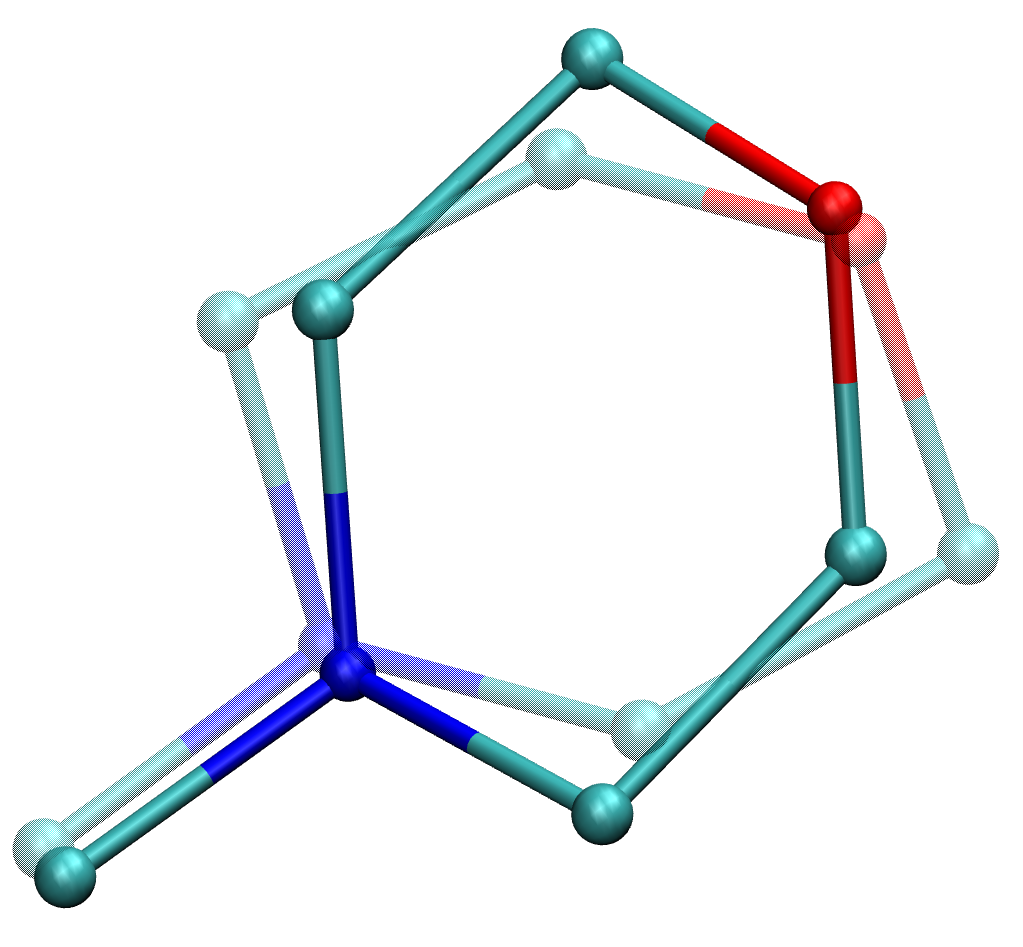
\includegraphics[width=\textwidth]{mode7_ot.png}
			\caption{mode 7: ``ring distortion"}
		\end{subfigure}
		\begin{subfigure}{\x\textwidth}
			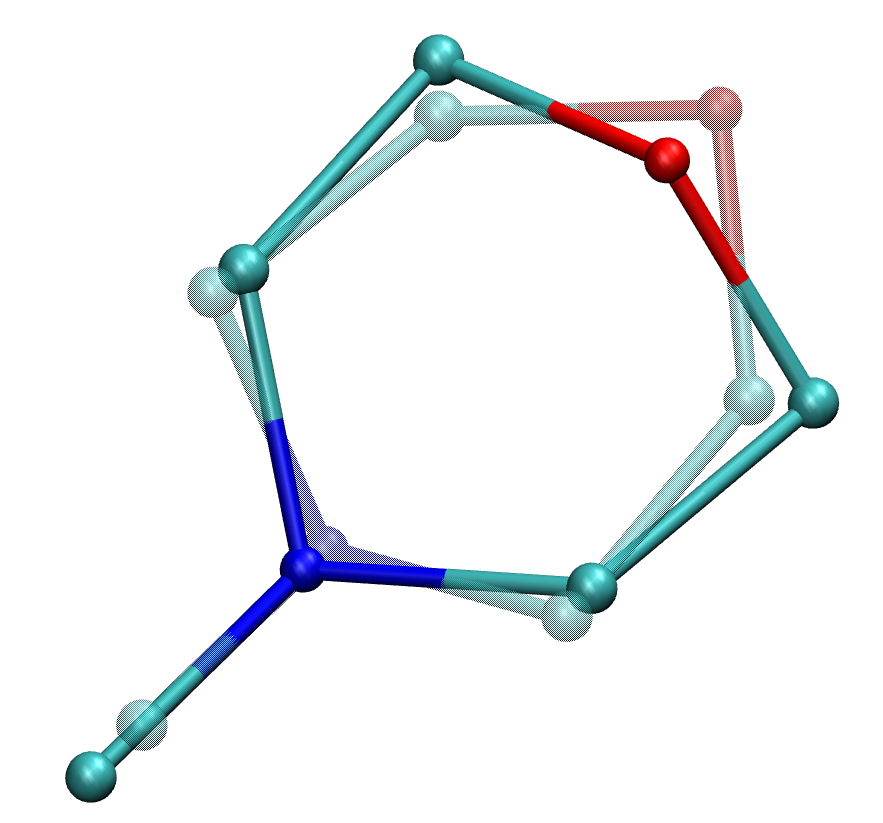
\includegraphics[width=\textwidth]{mode8_ot.png}
			\caption{mode 8: ``ring distortion"}
		\end{subfigure}
		\begin{subfigure}{\x\textwidth}
			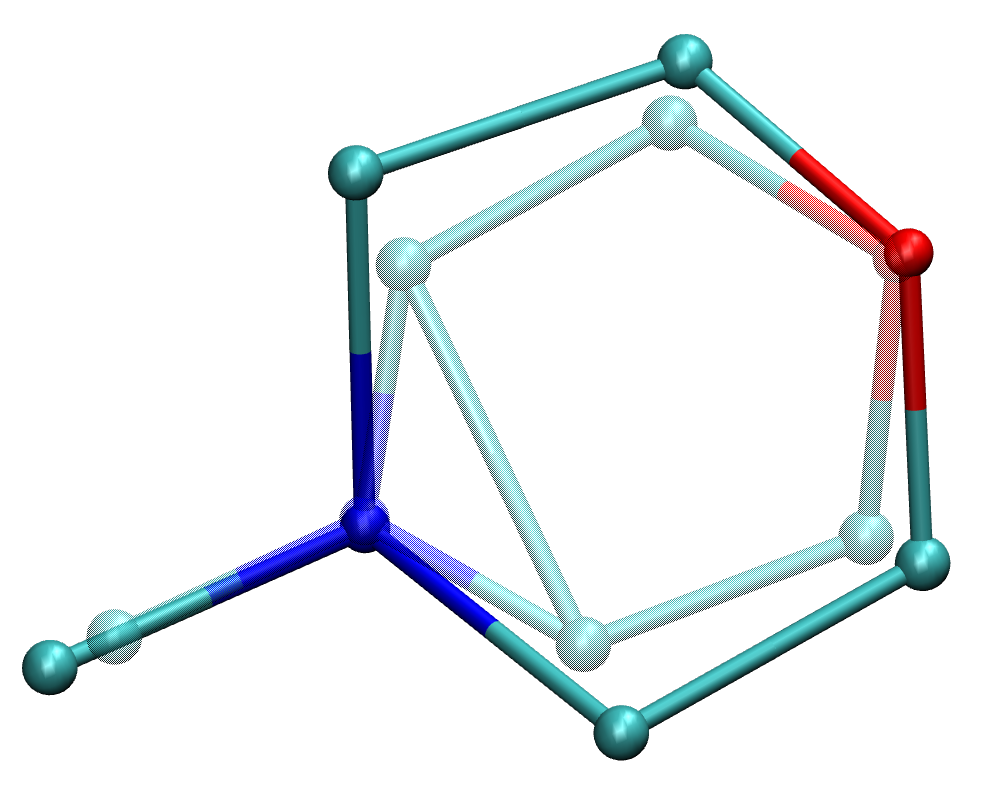
\includegraphics[width=\textwidth]{mode9_ot.png}
			\caption{mode 9: ``breathing"}
		\end{subfigure}
	\end{figure}
	$\dots (3N - 6 = 48)$
\end{frame}

%%% mode slides

\newcommand\m{0}
\newcommand{\molwidth}{0.1}
\newcommand{\vh}{-10}

%\iffalse
\iftrue

\begin{frame}{mode \m}
	\vspace{\vh mm}
	\begin{figure}
		\centering
		\includegraphics[width=\molwidth\textwidth]{mode\m_ot.png}
	\end{figure}
	\begin{figure}
		\centering
		\begin{subfigure}[b]{\w\textwidth}
			\centering
			\includegraphics[width=\textwidth]{../notebooks/100_mode\m_-0.10.png}
			\caption{-0.1 ps}
			\label{fig:}
		\end{subfigure}
		\begin{subfigure}[b]{\w\textwidth}
			\centering
			\includegraphics[width=\textwidth]{../notebooks/100_mode\m_-0.05.png}
			\caption{-0.05 ps}
			\label{fig:}
		\end{subfigure}
		\begin{subfigure}[b]{\w\textwidth}
			\centering
			\includegraphics[width=\textwidth]{../notebooks/100_mode\m_0.00.png}
			\caption{0 ps}
			\label{fig:}
		\end{subfigure}
		\begin{subfigure}[b]{\w\textwidth}
			\centering
			\includegraphics[width=\textwidth]{../notebooks/100_mode\m_0.05.png}
			\caption{0.05 ps}
			\label{fig:}
		\end{subfigure}
		\begin{subfigure}[b]{\w\textwidth}
			\centering
			\includegraphics[width=\textwidth]{../notebooks/100_mode\m_0.10.png}
			\caption{0.1 ps}
			\label{fig:}
		\end{subfigure}
		\begin{subfigure}[b]{\w\textwidth}
			\centering
			\includegraphics[width=\textwidth]{../notebooks/100_mode\m_1.00.png}
			\caption{1 ps}
			\label{fig:}
		\end{subfigure}
	\end{figure}
\end{frame}

\renewcommand\m{1}
\begin{frame}{mode \m}
	\vspace{\vh mm}
	\begin{figure}
		\centering
		\includegraphics[width=\molwidth\textwidth]{mode\m_ot.png}
	\end{figure}
	\begin{figure}
		\centering
		\begin{subfigure}[b]{\w\textwidth}
			\centering
			\includegraphics[width=\textwidth]{../notebooks/100_mode\m_-0.10.png}
			\caption{-0.1 ps}
		\end{subfigure}
		\begin{subfigure}[b]{\w\textwidth}
			\centering
			\includegraphics[width=\textwidth]{../notebooks/100_mode\m_-0.05.png}
			\caption{-0.05 ps}
		\end{subfigure}
		\begin{subfigure}[b]{\w\textwidth}
			\centering
			\includegraphics[width=\textwidth]{../notebooks/100_mode\m_0.00.png}
			\caption{0 ps}
		\end{subfigure}
		\begin{subfigure}[b]{\w\textwidth}
			\centering
			\includegraphics[width=\textwidth]{../notebooks/100_mode\m_0.05.png}
			\caption{0.05 ps}
		\end{subfigure}
		\begin{subfigure}[b]{\w\textwidth}
			\centering
			\includegraphics[width=\textwidth]{../notebooks/100_mode\m_0.10.png}
			\caption{0.1 ps}
		\end{subfigure}
		\begin{subfigure}[b]{\w\textwidth}
			\centering
			\includegraphics[width=\textwidth]{../notebooks/100_mode\m_1.00.png}
			\caption{1 ps}
		\end{subfigure}
	\end{figure}
\end{frame}

\renewcommand\m{2}

\begin{frame}{mode \m}
	\vspace{\vh mm}
		\begin{figure}
		\centering
		\includegraphics[width=\molwidth\textwidth]{mode\m_ot.png}
	\end{figure}
	\begin{figure}
		\centering
		\begin{subfigure}[b]{\w\textwidth}
			\centering
			\includegraphics[width=\textwidth]{../notebooks/100_mode\m_-0.10.png}
			\caption{-0.1 ps}
		\end{subfigure}
		\begin{subfigure}[b]{\w\textwidth}
			\centering
			\includegraphics[width=\textwidth]{../notebooks/100_mode\m_-0.05.png}
			\caption{-0.05 ps}
		\end{subfigure}
		\begin{subfigure}[b]{\w\textwidth}
			\centering
			\includegraphics[width=\textwidth]{../notebooks/100_mode\m_0.00.png}
			\caption{0 ps}
		\end{subfigure}
		\begin{subfigure}[b]{\w\textwidth}
			\centering
			\includegraphics[width=\textwidth]{../notebooks/100_mode\m_0.05.png}
			\caption{0.05 ps}
		\end{subfigure}
		\begin{subfigure}[b]{\w\textwidth}
			\centering
			\includegraphics[width=\textwidth]{../notebooks/100_mode\m_0.10.png}
			\caption{0.1 ps}
		\end{subfigure}
		\begin{subfigure}[b]{\w\textwidth}
			\centering
			\includegraphics[width=\textwidth]{../notebooks/100_mode\m_1.00.png}
			\caption{1 ps}
		\end{subfigure}
	\end{figure}
\end{frame}

\renewcommand\m{3}

\begin{frame}{mode \m}
	\vspace{\vh mm}
		\begin{figure}
		\centering
		\includegraphics[width=\molwidth\textwidth]{mode\m_ot.png}
	\end{figure}
	\begin{figure}
		\centering
		\begin{subfigure}[b]{\w\textwidth}
			\centering
			\includegraphics[width=\textwidth]{../notebooks/100_mode\m_-0.10.png}
			\caption{-0.1 ps}
		\end{subfigure}
		\begin{subfigure}[b]{\w\textwidth}
			\centering
			\includegraphics[width=\textwidth]{../notebooks/100_mode\m_-0.05.png}
			\caption{-0.05 ps}
		\end{subfigure}
		\begin{subfigure}[b]{\w\textwidth}
			\centering
			\includegraphics[width=\textwidth]{../notebooks/100_mode\m_0.00.png}
			\caption{0 ps}
		\end{subfigure}
		\begin{subfigure}[b]{\w\textwidth}
			\centering
			\includegraphics[width=\textwidth]{../notebooks/100_mode\m_0.05.png}
			\caption{0.05 ps}
		\end{subfigure}
		\begin{subfigure}[b]{\w\textwidth}
			\centering
			\includegraphics[width=\textwidth]{../notebooks/100_mode\m_0.10.png}
			\caption{0.1 ps}
		\end{subfigure}
		\begin{subfigure}[b]{\w\textwidth}
			\centering
			\includegraphics[width=\textwidth]{../notebooks/100_mode\m_1.00.png}
			\caption{1 ps}
		\end{subfigure}
	\end{figure}
\end{frame}

\renewcommand\m{4}

\begin{frame}{mode \m}
	\vspace{\vh mm}
		\begin{figure}
		\centering
		\includegraphics[width=\molwidth\textwidth]{mode\m_ot.png}
	\end{figure}
	\begin{figure}
		\centering
		\begin{subfigure}[b]{\w\textwidth}
			\centering
			\includegraphics[width=\textwidth]{../notebooks/100_mode\m_-0.10.png}
			\caption{-0.1 ps}
		\end{subfigure}
		\begin{subfigure}[b]{\w\textwidth}
			\centering
			\includegraphics[width=\textwidth]{../notebooks/100_mode\m_-0.05.png}
			\caption{-0.05 ps}
		\end{subfigure}
		\begin{subfigure}[b]{\w\textwidth}
			\centering
			\includegraphics[width=\textwidth]{../notebooks/100_mode\m_0.00.png}
			\caption{0 ps}
		\end{subfigure}
		\begin{subfigure}[b]{\w\textwidth}
			\centering
			\includegraphics[width=\textwidth]{../notebooks/100_mode\m_0.05.png}
			\caption{0.05 ps}
		\end{subfigure}
		\begin{subfigure}[b]{\w\textwidth}
			\centering
			\includegraphics[width=\textwidth]{../notebooks/100_mode\m_0.10.png}
			\caption{0.1 ps}
		\end{subfigure}
		\begin{subfigure}[b]{\w\textwidth}
			\centering
			\includegraphics[width=\textwidth]{../notebooks/100_mode\m_1.00.png}
			\caption{1 ps}
		\end{subfigure}
	\end{figure}
\end{frame}

\renewcommand\m{5}

\begin{frame}{mode \m}
	\vspace{\vh mm}
		\begin{figure}
		\centering
		\includegraphics[width=\molwidth\textwidth]{mode\m_ot.png}
	\end{figure}
	\begin{figure}
		\centering
		\begin{subfigure}[b]{\w\textwidth}
			\centering
			\includegraphics[width=\textwidth]{../notebooks/100_mode\m_-0.10.png}
			\caption{-0.1 ps}
		\end{subfigure}
		\begin{subfigure}[b]{\w\textwidth}
			\centering
			\includegraphics[width=\textwidth]{../notebooks/100_mode\m_-0.05.png}
			\caption{-0.05 ps}
		\end{subfigure}
		\begin{subfigure}[b]{\w\textwidth}
			\centering
			\includegraphics[width=\textwidth]{../notebooks/100_mode\m_0.00.png}
			\caption{0 ps}
		\end{subfigure}
		\begin{subfigure}[b]{\w\textwidth}
			\centering
			\includegraphics[width=\textwidth]{../notebooks/100_mode\m_0.05.png}
			\caption{0.05 ps}
		\end{subfigure}
		\begin{subfigure}[b]{\w\textwidth}
			\centering
			\includegraphics[width=\textwidth]{../notebooks/100_mode\m_0.10.png}
			\caption{0.1 ps}
		\end{subfigure}
		\begin{subfigure}[b]{\w\textwidth}
			\centering
			\includegraphics[width=\textwidth]{../notebooks/100_mode\m_1.00.png}
			\caption{1 ps}
		\end{subfigure}
	\end{figure}
\end{frame}

\renewcommand\m{6}
\begin{frame}{mode \m}
	\vspace{\vh mm}
	\begin{figure}
		\centering
		\includegraphics[width=\molwidth\textwidth]{mode\m_ot.png}
	\end{figure}
	\begin{figure}
		\centering
		\begin{subfigure}[b]{\w\textwidth}
			\centering
			\includegraphics[width=\textwidth]{../notebooks/100_mode\m_-0.10.png}
			\caption{-0.1 ps}
		\end{subfigure}
		\begin{subfigure}[b]{\w\textwidth}
			\centering
			\includegraphics[width=\textwidth]{../notebooks/100_mode\m_-0.05.png}
			\caption{-0.05 ps}
		\end{subfigure}
		\begin{subfigure}[b]{\w\textwidth}
			\centering
			\includegraphics[width=\textwidth]{../notebooks/100_mode\m_0.00.png}
			\caption{0 ps}
		\end{subfigure}
		\begin{subfigure}[b]{\w\textwidth}
			\centering
			\includegraphics[width=\textwidth]{../notebooks/100_mode\m_0.05.png}
			\caption{0.05 ps}
		\end{subfigure}
		\begin{subfigure}[b]{\w\textwidth}
			\centering
			\includegraphics[width=\textwidth]{../notebooks/100_mode\m_0.10.png}
			\caption{0.1 ps}
		\end{subfigure}
		\begin{subfigure}[b]{\w\textwidth}
			\centering
			\includegraphics[width=\textwidth]{../notebooks/100_mode\m_1.00.png}
			\caption{1 ps}
		\end{subfigure}
	\end{figure}
\end{frame}

\renewcommand\m{7}

\begin{frame}{mode \m}
	\vspace{\vh mm}
	\begin{figure}
		\centering
		\includegraphics[width=\molwidth\textwidth]{mode\m_ot.png}
	\end{figure}
	\begin{figure}
		\centering
		\begin{subfigure}[b]{\w\textwidth}
			\centering
			\includegraphics[width=\textwidth]{../notebooks/100_mode\m_-0.10.png}
			\caption{-0.1 ps}
		\end{subfigure}
		\begin{subfigure}[b]{\w\textwidth}
			\centering
			\includegraphics[width=\textwidth]{../notebooks/100_mode\m_-0.05.png}
			\caption{-0.05 ps}
		\end{subfigure}
		\begin{subfigure}[b]{\w\textwidth}
			\centering
			\includegraphics[width=\textwidth]{../notebooks/100_mode\m_0.00.png}
			\caption{0 ps}
		\end{subfigure}
		\begin{subfigure}[b]{\w\textwidth}
			\centering
			\includegraphics[width=\textwidth]{../notebooks/100_mode\m_0.05.png}
			\caption{0.05 ps}
		\end{subfigure}
		\begin{subfigure}[b]{\w\textwidth}
			\centering
			\includegraphics[width=\textwidth]{../notebooks/100_mode\m_0.10.png}
			\caption{0.1 ps}
		\end{subfigure}
		\begin{subfigure}[b]{\w\textwidth}
			\centering
			\includegraphics[width=\textwidth]{../notebooks/100_mode\m_1.00.png}
			\caption{1 ps}
		\end{subfigure}
	\end{figure}
\end{frame}

\renewcommand\m{8}
\begin{frame}{mode \m}
	\vspace{\vh mm}
\begin{figure}
	\centering
	\includegraphics[width=\molwidth\textwidth]{mode\m_ot.png}
\end{figure}
	\begin{figure}
		\centering
		\begin{subfigure}[b]{\w\textwidth}
			\centering
			\includegraphics[width=\textwidth]{../notebooks/100_mode\m_-0.10.png}
			\caption{-0.1 ps}
		\end{subfigure}
		\begin{subfigure}[b]{\w\textwidth}
			\centering
			\includegraphics[width=\textwidth]{../notebooks/100_mode\m_-0.05.png}
			\caption{-0.05 ps}
		\end{subfigure}
		\begin{subfigure}[b]{\w\textwidth}
			\centering
			\includegraphics[width=\textwidth]{../notebooks/100_mode\m_0.00.png}
			\caption{0 ps}
		\end{subfigure}
		\begin{subfigure}[b]{\w\textwidth}
			\centering
			\includegraphics[width=\textwidth]{../notebooks/100_mode\m_0.05.png}
			\caption{0.05 ps}
		\end{subfigure}
		\begin{subfigure}[b]{\w\textwidth}
			\centering
			\includegraphics[width=\textwidth]{../notebooks/100_mode\m_0.10.png}
			\caption{0.1 ps}
		\end{subfigure}
		\begin{subfigure}[b]{\w\textwidth}
			\centering
			\includegraphics[width=\textwidth]{../notebooks/100_mode\m_1.00.png}
			\caption{1 ps}
		\end{subfigure}
	\end{figure}
\end{frame}

\renewcommand\m{9}
\begin{frame}{mode \m}
	\vspace{\vh mm}
\begin{figure}
	\centering
	\includegraphics[width=\molwidth\textwidth]{mode\m_ot.png}
\end{figure}
	\begin{figure}
		\centering
		\begin{subfigure}[b]{\w\textwidth}
			\centering
			\includegraphics[width=\textwidth]{../notebooks/100_mode\m_-0.10.png}
			\caption{-0.1 ps}
		\end{subfigure}
		\begin{subfigure}[b]{\w\textwidth}
			\centering
			\includegraphics[width=\textwidth]{../notebooks/100_mode\m_-0.05.png}
			\caption{-0.05 ps}
		\end{subfigure}
		\begin{subfigure}[b]{\w\textwidth}
			\centering
			\includegraphics[width=\textwidth]{../notebooks/100_mode\m_0.00.png}
			\caption{0 ps}
		\end{subfigure}
		\begin{subfigure}[b]{\w\textwidth}
			\centering
			\includegraphics[width=\textwidth]{../notebooks/100_mode\m_0.05.png}
			\caption{0.05 ps}
		\end{subfigure}
		\begin{subfigure}[b]{\w\textwidth}
			\centering
			\includegraphics[width=\textwidth]{../notebooks/100_mode\m_0.10.png}
			\caption{0.1 ps}
		\end{subfigure}
		\begin{subfigure}[b]{\w\textwidth}
			\centering
			\includegraphics[width=\textwidth]{../notebooks/100_mode\m_1.00.png}
			\caption{1 ps}
		\end{subfigure}
	\end{figure}
\end{frame}

\renewcommand\m{10}
\begin{frame}{mode \m}
		\vspace{\vh mm}
	\begin{figure}
		\centering
		\includegraphics[width=\molwidth\textwidth]{mode\m_ot.png}
	\end{figure}
	\begin{figure}
		\centering
		\begin{subfigure}[b]{\w\textwidth}
			\centering
			\includegraphics[width=\textwidth]{../notebooks/100_mode\m_-0.10.png}
			\caption{-0.1 ps}
		\end{subfigure}
		\begin{subfigure}[b]{\w\textwidth}
			\centering
			\includegraphics[width=\textwidth]{../notebooks/100_mode\m_-0.05.png}
			\caption{-0.05 ps}
		\end{subfigure}
		\begin{subfigure}[b]{\w\textwidth}
			\centering
			\includegraphics[width=\textwidth]{../notebooks/100_mode\m_0.00.png}
			\caption{0 ps}
		\end{subfigure}
		\begin{subfigure}[b]{\w\textwidth}
			\centering
			\includegraphics[width=\textwidth]{../notebooks/100_mode\m_0.05.png}
			\caption{0.05 ps}
		\end{subfigure}
		\begin{subfigure}[b]{\w\textwidth}
			\centering
			\includegraphics[width=\textwidth]{../notebooks/100_mode\m_0.10.png}
			\caption{0.1 ps}
		\end{subfigure}
		\begin{subfigure}[b]{\w\textwidth}
			\centering
			\includegraphics[width=\textwidth]{../notebooks/100_mode\m_1.00.png}
			\caption{1 ps}
		\end{subfigure}
	\end{figure}
\end{frame}

\renewcommand\m{11}
\begin{frame}{mode \m}
		\vspace{\vh mm}
	\begin{figure}
		\centering
		\includegraphics[width=\molwidth\textwidth]{mode\m_ot.png}
	\end{figure}
	\begin{figure}
		\centering
		\begin{subfigure}[b]{\w\textwidth}
			\centering
			\includegraphics[width=\textwidth]{../notebooks/100_mode\m_-0.10.png}
			\caption{-0.1 ps}
		\end{subfigure}
		\begin{subfigure}[b]{\w\textwidth}
			\centering
			\includegraphics[width=\textwidth]{../notebooks/100_mode\m_-0.05.png}
			\caption{-0.05 ps}
		\end{subfigure}
		\begin{subfigure}[b]{\w\textwidth}
			\centering
			\includegraphics[width=\textwidth]{../notebooks/100_mode\m_0.00.png}
			\caption{0 ps}
		\end{subfigure}
		\begin{subfigure}[b]{\w\textwidth}
			\centering
			\includegraphics[width=\textwidth]{../notebooks/100_mode\m_0.05.png}
			\caption{0.05 ps}
		\end{subfigure}
		\begin{subfigure}[b]{\w\textwidth}
			\centering
			\includegraphics[width=\textwidth]{../notebooks/100_mode\m_0.10.png}
			\caption{0.1 ps}
		\end{subfigure}
		\begin{subfigure}[b]{\w\textwidth}
			\centering
			\includegraphics[width=\textwidth]{../notebooks/100_mode\m_1.00.png}
			\caption{1 ps}
		\end{subfigure}
	\end{figure}
\end{frame}

\renewcommand\m{12}
\begin{frame}{mode \m}
		\vspace{\vh mm}
	\begin{figure}
		\centering
		\includegraphics[width=\molwidth\textwidth]{mode\m_ot.png}
	\end{figure}
	\begin{figure}
		\centering
		\begin{subfigure}[b]{\w\textwidth}
			\centering
			\includegraphics[width=\textwidth]{../notebooks/100_mode\m_-0.10.png}
			\caption{-0.1 ps}
		\end{subfigure}
		\begin{subfigure}[b]{\w\textwidth}
			\centering
			\includegraphics[width=\textwidth]{../notebooks/100_mode\m_-0.05.png}
			\caption{-0.05 ps}
		\end{subfigure}
		\begin{subfigure}[b]{\w\textwidth}
			\centering
			\includegraphics[width=\textwidth]{../notebooks/100_mode\m_0.00.png}
			\caption{0 ps}
		\end{subfigure}
		\begin{subfigure}[b]{\w\textwidth}
			\centering
			\includegraphics[width=\textwidth]{../notebooks/100_mode\m_0.05.png}
			\caption{0.05 ps}
		\end{subfigure}
		\begin{subfigure}[b]{\w\textwidth}
			\centering
			\includegraphics[width=\textwidth]{../notebooks/100_mode\m_0.10.png}
			\caption{0.1 ps}
		\end{subfigure}
		\begin{subfigure}[b]{\w\textwidth}
			\centering
			\includegraphics[width=\textwidth]{../notebooks/100_mode\m_1.00.png}
			\caption{1 ps}
		\end{subfigure}
	\end{figure}
\end{frame}

\renewcommand\m{13}
\begin{frame}{mode \m}
		\vspace{\vh mm}
	\begin{figure}
		\centering
		\includegraphics[width=\molwidth\textwidth]{mode\m_ot.png}
	\end{figure}
	\begin{figure}
		\centering
		\begin{subfigure}[b]{\w\textwidth}
			\centering
			\includegraphics[width=\textwidth]{../notebooks/100_mode\m_-0.10.png}
			\caption{-0.1 ps}
		\end{subfigure}
		\begin{subfigure}[b]{\w\textwidth}
			\centering
			\includegraphics[width=\textwidth]{../notebooks/100_mode\m_-0.05.png}
			\caption{-0.05 ps}
		\end{subfigure}
		\begin{subfigure}[b]{\w\textwidth}
			\centering
			\includegraphics[width=\textwidth]{../notebooks/100_mode\m_0.00.png}
			\caption{0 ps}
		\end{subfigure}
		\begin{subfigure}[b]{\w\textwidth}
			\centering
			\includegraphics[width=\textwidth]{../notebooks/100_mode\m_0.05.png}
			\caption{0.05 ps}
		\end{subfigure}
		\begin{subfigure}[b]{\w\textwidth}
			\centering
			\includegraphics[width=\textwidth]{../notebooks/100_mode\m_0.10.png}
			\caption{0.1 ps}
		\end{subfigure}
		\begin{subfigure}[b]{\w\textwidth}
			\centering
			\includegraphics[width=\textwidth]{../notebooks/100_mode\m_1.00.png}
			\caption{1 ps}
		\end{subfigure}
	\end{figure}
\end{frame}

\renewcommand\m{14}
\begin{frame}{mode \m}
		\vspace{\vh mm}
	\begin{figure}
		\centering
		\includegraphics[width=\molwidth\textwidth]{mode\m_ot.png}
	\end{figure}
	\begin{figure}
		\centering
		\begin{subfigure}[b]{\w\textwidth}
			\centering
			\includegraphics[width=\textwidth]{../notebooks/100_mode\m_-0.10.png}
			\caption{-0.1 ps}
		\end{subfigure}
		\begin{subfigure}[b]{\w\textwidth}
			\centering
			\includegraphics[width=\textwidth]{../notebooks/100_mode\m_-0.05.png}
			\caption{-0.05 ps}
		\end{subfigure}
		\begin{subfigure}[b]{\w\textwidth}
			\centering
			\includegraphics[width=\textwidth]{../notebooks/100_mode\m_0.00.png}
			\caption{0 ps}
		\end{subfigure}
		\begin{subfigure}[b]{\w\textwidth}
			\centering
			\includegraphics[width=\textwidth]{../notebooks/100_mode\m_0.05.png}
			\caption{0.05 ps}
		\end{subfigure}
		\begin{subfigure}[b]{\w\textwidth}
			\centering
			\includegraphics[width=\textwidth]{../notebooks/100_mode\m_0.10.png}
			\caption{0.1 ps}
		\end{subfigure}
		\begin{subfigure}[b]{\w\textwidth}
			\centering
			\includegraphics[width=\textwidth]{../notebooks/100_mode\m_1.00.png}
			\caption{1 ps}
		\end{subfigure}
	\end{figure}
\end{frame}

\renewcommand\m{15}
\begin{frame}{mode \m}
			\vspace{\vh mm}
	\begin{figure}
		\centering
		\includegraphics[width=\molwidth\textwidth]{mode\m_ot.png}
	\end{figure}
	\begin{figure}
		\centering
		\begin{subfigure}[b]{\w\textwidth}
			\centering
			\includegraphics[width=\textwidth]{../notebooks/100_mode\m_-0.10.png}
			\caption{-0.1 ps}
		\end{subfigure}
		\begin{subfigure}[b]{\w\textwidth}
			\centering
			\includegraphics[width=\textwidth]{../notebooks/100_mode\m_-0.05.png}
			\caption{-0.05 ps}
		\end{subfigure}
		\begin{subfigure}[b]{\w\textwidth}
			\centering
			\includegraphics[width=\textwidth]{../notebooks/100_mode\m_0.00.png}
			\caption{0 ps}
		\end{subfigure}
		\begin{subfigure}[b]{\w\textwidth}
			\centering
			\includegraphics[width=\textwidth]{../notebooks/100_mode\m_0.05.png}
			\caption{0.05 ps}
		\end{subfigure}
		\begin{subfigure}[b]{\w\textwidth}
			\centering
			\includegraphics[width=\textwidth]{../notebooks/100_mode\m_0.10.png}
			\caption{0.1 ps}
		\end{subfigure}
		\begin{subfigure}[b]{\w\textwidth}
			\centering
			\includegraphics[width=\textwidth]{../notebooks/100_mode\m_1.00.png}
			\caption{1 ps}
		\end{subfigure}
	\end{figure}
\end{frame}

\renewcommand\m{16}
\begin{frame}{mode \m}
			\vspace{\vh mm}
	\begin{figure}
		\centering
		\includegraphics[width=\molwidth\textwidth]{mode\m_ot.png}
	\end{figure}
	\begin{figure}
		\centering
		\begin{subfigure}[b]{\w\textwidth}
			\centering
			\includegraphics[width=\textwidth]{../notebooks/100_mode\m_-0.10.png}
			\caption{-0.1 ps}
		\end{subfigure}
		\begin{subfigure}[b]{\w\textwidth}
			\centering
			\includegraphics[width=\textwidth]{../notebooks/100_mode\m_-0.05.png}
			\caption{-0.05 ps}
		\end{subfigure}
		\begin{subfigure}[b]{\w\textwidth}
			\centering
			\includegraphics[width=\textwidth]{../notebooks/100_mode\m_0.00.png}
			\caption{0 ps}
		\end{subfigure}
		\begin{subfigure}[b]{\w\textwidth}
			\centering
			\includegraphics[width=\textwidth]{../notebooks/100_mode\m_0.05.png}
			\caption{0.05 ps}
		\end{subfigure}
		\begin{subfigure}[b]{\w\textwidth}
			\centering
			\includegraphics[width=\textwidth]{../notebooks/100_mode\m_0.10.png}
			\caption{0.1 ps}
		\end{subfigure}
		\begin{subfigure}[b]{\w\textwidth}
			\centering
			\includegraphics[width=\textwidth]{../notebooks/100_mode\m_1.00.png}
			\caption{1 ps}
		\end{subfigure}
	\end{figure}
\end{frame}

\renewcommand\m{17}
\begin{frame}{mode \m}
				\vspace{\vh mm}
	\begin{figure}
		\centering
		\includegraphics[width=\molwidth\textwidth]{mode\m_ot.png}
	\end{figure}
	\begin{figure}
		\centering
		\begin{subfigure}[b]{\w\textwidth}
			\centering
			\includegraphics[width=\textwidth]{../notebooks/100_mode\m_-0.10.png}
			\caption{-0.1 ps}
		\end{subfigure}
		\begin{subfigure}[b]{\w\textwidth}
			\centering
			\includegraphics[width=\textwidth]{../notebooks/100_mode\m_-0.05.png}
			\caption{-0.05 ps}
		\end{subfigure}
		\begin{subfigure}[b]{\w\textwidth}
			\centering
			\includegraphics[width=\textwidth]{../notebooks/100_mode\m_0.00.png}
			\caption{0 ps}
		\end{subfigure}
		\begin{subfigure}[b]{\w\textwidth}
			\centering
			\includegraphics[width=\textwidth]{../notebooks/100_mode\m_0.05.png}
			\caption{0.05 ps}
		\end{subfigure}
		\begin{subfigure}[b]{\w\textwidth}
			\centering
			\includegraphics[width=\textwidth]{../notebooks/100_mode\m_0.10.png}
			\caption{0.1 ps}
		\end{subfigure}
		\begin{subfigure}[b]{\w\textwidth}
			\centering
			\includegraphics[width=\textwidth]{../notebooks/100_mode\m_1.00.png}
			\caption{1 ps}
		\end{subfigure}
	\end{figure}
\end{frame}

\renewcommand\m{18}
\begin{frame}{mode \m}
				\vspace{\vh mm}
	\begin{figure}
		\centering
		\includegraphics[width=\molwidth\textwidth]{mode\m_ot.png}
	\end{figure}
	\begin{figure}
		\centering
		\begin{subfigure}[b]{\w\textwidth}
			\centering
			\includegraphics[width=\textwidth]{../notebooks/100_mode\m_-0.10.png}
			\caption{-0.1 ps}
		\end{subfigure}
		\begin{subfigure}[b]{\w\textwidth}
			\centering
			\includegraphics[width=\textwidth]{../notebooks/100_mode\m_-0.05.png}
			\caption{-0.05 ps}
		\end{subfigure}
		\begin{subfigure}[b]{\w\textwidth}
			\centering
			\includegraphics[width=\textwidth]{../notebooks/100_mode\m_0.00.png}
			\caption{0 ps}
		\end{subfigure}
		\begin{subfigure}[b]{\w\textwidth}
			\centering
			\includegraphics[width=\textwidth]{../notebooks/100_mode\m_0.05.png}
			\caption{0.05 ps}
		\end{subfigure}
		\begin{subfigure}[b]{\w\textwidth}
			\centering
			\includegraphics[width=\textwidth]{../notebooks/100_mode\m_0.10.png}
			\caption{0.1 ps}
		\end{subfigure}
		\begin{subfigure}[b]{\w\textwidth}
			\centering
			\includegraphics[width=\textwidth]{../notebooks/100_mode\m_1.00.png}
			\caption{1 ps}
		\end{subfigure}
	\end{figure}
\end{frame}

\renewcommand\m{19}
\begin{frame}{mode \m}
					\vspace{\vh mm}
	\begin{figure}
		\centering
		\includegraphics[width=\molwidth\textwidth]{mode\m_ot.png}
	\end{figure}
	\begin{figure}
		\centering
		\begin{subfigure}[b]{\w\textwidth}
			\centering
			\includegraphics[width=\textwidth]{../notebooks/100_mode\m_-0.10.png}
			\caption{-0.1 ps}
		\end{subfigure}
		\begin{subfigure}[b]{\w\textwidth}
			\centering
			\includegraphics[width=\textwidth]{../notebooks/100_mode\m_-0.05.png}
			\caption{-0.05 ps}
		\end{subfigure}
		\begin{subfigure}[b]{\w\textwidth}
			\centering
			\includegraphics[width=\textwidth]{../notebooks/100_mode\m_0.00.png}
			\caption{0 ps}
		\end{subfigure}
		\begin{subfigure}[b]{\w\textwidth}
			\centering
			\includegraphics[width=\textwidth]{../notebooks/100_mode\m_0.05.png}
			\caption{0.05 ps}
		\end{subfigure}
		\begin{subfigure}[b]{\w\textwidth}
			\centering
			\includegraphics[width=\textwidth]{../notebooks/100_mode\m_0.10.png}
			\caption{0.1 ps}
		\end{subfigure}
		\begin{subfigure}[b]{\w\textwidth}
			\centering
			\includegraphics[width=\textwidth]{../notebooks/100_mode\m_1.00.png}
			\caption{1 ps}
		\end{subfigure}
	\end{figure}
\end{frame}

\renewcommand\m{20}
\begin{frame}{mode \m}
					\vspace{\vh mm}
	\begin{figure}
		\centering
		\includegraphics[width=\molwidth\textwidth]{mode\m_ot.png}
	\end{figure}
	\begin{figure}
		\centering
		\begin{subfigure}[b]{\w\textwidth}
			\centering
			\includegraphics[width=\textwidth]{../notebooks/100_mode\m_-0.10.png}
			\caption{-0.1 ps}
		\end{subfigure}
		\begin{subfigure}[b]{\w\textwidth}
			\centering
			\includegraphics[width=\textwidth]{../notebooks/100_mode\m_-0.05.png}
			\caption{-0.05 ps}
		\end{subfigure}
		\begin{subfigure}[b]{\w\textwidth}
			\centering
			\includegraphics[width=\textwidth]{../notebooks/100_mode\m_0.00.png}
			\caption{0 ps}
		\end{subfigure}
		\begin{subfigure}[b]{\w\textwidth}
			\centering
			\includegraphics[width=\textwidth]{../notebooks/100_mode\m_0.05.png}
			\caption{0.05 ps}
		\end{subfigure}
		\begin{subfigure}[b]{\w\textwidth}
			\centering
			\includegraphics[width=\textwidth]{../notebooks/100_mode\m_0.10.png}
			\caption{0.1 ps}
		\end{subfigure}
		\begin{subfigure}[b]{\w\textwidth}
			\centering
			\includegraphics[width=\textwidth]{../notebooks/100_mode\m_1.00.png}
			\caption{1 ps}
		\end{subfigure}
	\end{figure}
\end{frame}

\renewcommand\m{21}
\begin{frame}{mode \m}
	\begin{figure}
		\centering
		\begin{subfigure}[b]{\w\textwidth}
			\centering
			\includegraphics[width=\textwidth]{../notebooks/100_mode\m_-0.10.png}
			\caption{-0.1 ps}
		\end{subfigure}
		\begin{subfigure}[b]{\w\textwidth}
			\centering
			\includegraphics[width=\textwidth]{../notebooks/100_mode\m_-0.05.png}
			\caption{-0.05 ps}
		\end{subfigure}
		\begin{subfigure}[b]{\w\textwidth}
			\centering
			\includegraphics[width=\textwidth]{../notebooks/100_mode\m_0.00.png}
			\caption{0 ps}
		\end{subfigure}
		\begin{subfigure}[b]{\w\textwidth}
			\centering
			\includegraphics[width=\textwidth]{../notebooks/100_mode\m_0.05.png}
			\caption{0.05 ps}
		\end{subfigure}
		\begin{subfigure}[b]{\w\textwidth}
			\centering
			\includegraphics[width=\textwidth]{../notebooks/100_mode\m_0.10.png}
			\caption{0.1 ps}
		\end{subfigure}
		\begin{subfigure}[b]{\w\textwidth}
			\centering
			\includegraphics[width=\textwidth]{../notebooks/100_mode\m_1.00.png}
			\caption{1 ps}
		\end{subfigure}
	\end{figure}
\end{frame}

\renewcommand\m{22}
\begin{frame}{mode \m}
	\begin{figure}
		\centering
		\begin{subfigure}[b]{\w\textwidth}
			\centering
			\includegraphics[width=\textwidth]{../notebooks/100_mode\m_-0.10.png}
			\caption{-0.1 ps}
		\end{subfigure}
		\begin{subfigure}[b]{\w\textwidth}
			\centering
			\includegraphics[width=\textwidth]{../notebooks/100_mode\m_-0.05.png}
			\caption{-0.05 ps}
		\end{subfigure}
		\begin{subfigure}[b]{\w\textwidth}
			\centering
			\includegraphics[width=\textwidth]{../notebooks/100_mode\m_0.00.png}
			\caption{0 ps}
		\end{subfigure}
		\begin{subfigure}[b]{\w\textwidth}
			\centering
			\includegraphics[width=\textwidth]{../notebooks/100_mode\m_0.05.png}
			\caption{0.05 ps}
		\end{subfigure}
		\begin{subfigure}[b]{\w\textwidth}
			\centering
			\includegraphics[width=\textwidth]{../notebooks/100_mode\m_0.10.png}
			\caption{0.1 ps}
		\end{subfigure}
		\begin{subfigure}[b]{\w\textwidth}
			\centering
			\includegraphics[width=\textwidth]{../notebooks/100_mode\m_1.00.png}
			\caption{1 ps}
		\end{subfigure}
	\end{figure}
\end{frame}

\renewcommand\m{23}
\begin{frame}{mode \m}
	\begin{figure}
		\centering
		\begin{subfigure}[b]{\w\textwidth}
			\centering
			\includegraphics[width=\textwidth]{../notebooks/100_mode\m_-0.10.png}
			\caption{-0.1 ps}
		\end{subfigure}
		\begin{subfigure}[b]{\w\textwidth}
			\centering
			\includegraphics[width=\textwidth]{../notebooks/100_mode\m_-0.05.png}
			\caption{-0.05 ps}
		\end{subfigure}
		\begin{subfigure}[b]{\w\textwidth}
			\centering
			\includegraphics[width=\textwidth]{../notebooks/100_mode\m_0.00.png}
			\caption{0 ps}
		\end{subfigure}
		\begin{subfigure}[b]{\w\textwidth}
			\centering
			\includegraphics[width=\textwidth]{../notebooks/100_mode\m_0.05.png}
			\caption{0.05 ps}
		\end{subfigure}
		\begin{subfigure}[b]{\w\textwidth}
			\centering
			\includegraphics[width=\textwidth]{../notebooks/100_mode\m_0.10.png}
			\caption{0.1 ps}
		\end{subfigure}
		\begin{subfigure}[b]{\w\textwidth}
			\centering
			\includegraphics[width=\textwidth]{../notebooks/100_mode\m_1.00.png}
			\caption{1 ps}
		\end{subfigure}
	\end{figure}
\end{frame}

\renewcommand\m{24}
\begin{frame}{mode \m}
	\begin{figure}
		\centering
		\begin{subfigure}[b]{\w\textwidth}
			\centering
			\includegraphics[width=\textwidth]{../notebooks/100_mode\m_-0.10.png}
			\caption{-0.1 ps}
		\end{subfigure}
		\begin{subfigure}[b]{\w\textwidth}
			\centering
			\includegraphics[width=\textwidth]{../notebooks/100_mode\m_-0.05.png}
			\caption{-0.05 ps}
		\end{subfigure}
		\begin{subfigure}[b]{\w\textwidth}
			\centering
			\includegraphics[width=\textwidth]{../notebooks/100_mode\m_0.00.png}
			\caption{0 ps}
		\end{subfigure}
		\begin{subfigure}[b]{\w\textwidth}
			\centering
			\includegraphics[width=\textwidth]{../notebooks/100_mode\m_0.05.png}
			\caption{0.05 ps}
		\end{subfigure}
		\begin{subfigure}[b]{\w\textwidth}
			\centering
			\includegraphics[width=\textwidth]{../notebooks/100_mode\m_0.10.png}
			\caption{0.1 ps}
		\end{subfigure}
		\begin{subfigure}[b]{\w\textwidth}
			\centering
			\includegraphics[width=\textwidth]{../notebooks/100_mode\m_1.00.png}
			\caption{1 ps}
		\end{subfigure}
	\end{figure}
\end{frame}

\renewcommand\m{25}
\begin{frame}{mode \m}
	\begin{figure}
		\centering
		\begin{subfigure}[b]{\w\textwidth}
			\centering
			\includegraphics[width=\textwidth]{../notebooks/100_mode\m_-0.10.png}
			\caption{-0.1 ps}
		\end{subfigure}
		\begin{subfigure}[b]{\w\textwidth}
			\centering
			\includegraphics[width=\textwidth]{../notebooks/100_mode\m_-0.05.png}
			\caption{-0.05 ps}
		\end{subfigure}
		\begin{subfigure}[b]{\w\textwidth}
			\centering
			\includegraphics[width=\textwidth]{../notebooks/100_mode\m_0.00.png}
			\caption{0 ps}
		\end{subfigure}
		\begin{subfigure}[b]{\w\textwidth}
			\centering
			\includegraphics[width=\textwidth]{../notebooks/100_mode\m_0.05.png}
			\caption{0.05 ps}
		\end{subfigure}
		\begin{subfigure}[b]{\w\textwidth}
			\centering
			\includegraphics[width=\textwidth]{../notebooks/100_mode\m_0.10.png}
			\caption{0.1 ps}
		\end{subfigure}
		\begin{subfigure}[b]{\w\textwidth}
			\centering
			\includegraphics[width=\textwidth]{../notebooks/100_mode\m_1.00.png}
			\caption{1 ps}
		\end{subfigure}
	\end{figure}
\end{frame}

\renewcommand\m{26}
\begin{frame}{mode \m}
	\begin{figure}
		\centering
		\begin{subfigure}[b]{\w\textwidth}
			\centering
			\includegraphics[width=\textwidth]{../notebooks/100_mode\m_-0.10.png}
			\caption{-0.1 ps}
		\end{subfigure}
		\begin{subfigure}[b]{\w\textwidth}
			\centering
			\includegraphics[width=\textwidth]{../notebooks/100_mode\m_-0.05.png}
			\caption{-0.05 ps}
		\end{subfigure}
		\begin{subfigure}[b]{\w\textwidth}
			\centering
			\includegraphics[width=\textwidth]{../notebooks/100_mode\m_0.00.png}
			\caption{0 ps}
		\end{subfigure}
		\begin{subfigure}[b]{\w\textwidth}
			\centering
			\includegraphics[width=\textwidth]{../notebooks/100_mode\m_0.05.png}
			\caption{0.05 ps}
		\end{subfigure}
		\begin{subfigure}[b]{\w\textwidth}
			\centering
			\includegraphics[width=\textwidth]{../notebooks/100_mode\m_0.10.png}
			\caption{0.1 ps}
		\end{subfigure}
		\begin{subfigure}[b]{\w\textwidth}
			\centering
			\includegraphics[width=\textwidth]{../notebooks/100_mode\m_1.00.png}
			\caption{1 ps}
		\end{subfigure}
	\end{figure}
\end{frame}

\renewcommand\m{27}
\begin{frame}{mode \m}
	\begin{figure}
		\centering
		\begin{subfigure}[b]{\w\textwidth}
			\centering
			\includegraphics[width=\textwidth]{../notebooks/100_mode\m_-0.10.png}
			\caption{-0.1 ps}
		\end{subfigure}
		\begin{subfigure}[b]{\w\textwidth}
			\centering
			\includegraphics[width=\textwidth]{../notebooks/100_mode\m_-0.05.png}
			\caption{-0.05 ps}
		\end{subfigure}
		\begin{subfigure}[b]{\w\textwidth}
			\centering
			\includegraphics[width=\textwidth]{../notebooks/100_mode\m_0.00.png}
			\caption{0 ps}
		\end{subfigure}
		\begin{subfigure}[b]{\w\textwidth}
			\centering
			\includegraphics[width=\textwidth]{../notebooks/100_mode\m_0.05.png}
			\caption{0.05 ps}
		\end{subfigure}
		\begin{subfigure}[b]{\w\textwidth}
			\centering
			\includegraphics[width=\textwidth]{../notebooks/100_mode\m_0.10.png}
			\caption{0.1 ps}
		\end{subfigure}
		\begin{subfigure}[b]{\w\textwidth}
			\centering
			\includegraphics[width=\textwidth]{../notebooks/100_mode\m_1.00.png}
			\caption{1 ps}
		\end{subfigure}
	\end{figure}
\end{frame}

\renewcommand\m{28}
\begin{frame}{mode \m}
					\vspace{\vh mm}
	\begin{figure}
		\centering
		\includegraphics[width=\molwidth\textwidth]{mode\m_ot.png}
	\end{figure}
	\begin{figure}
		\centering
		\begin{subfigure}[b]{\w\textwidth}
			\centering
			\includegraphics[width=\textwidth]{../notebooks/100_mode\m_-0.10.png}
			\caption{-0.1 ps}
		\end{subfigure}
		\begin{subfigure}[b]{\w\textwidth}
			\centering
			\includegraphics[width=\textwidth]{../notebooks/100_mode\m_-0.05.png}
			\caption{-0.05 ps}
		\end{subfigure}
		\begin{subfigure}[b]{\w\textwidth}
			\centering
			\includegraphics[width=\textwidth]{../notebooks/100_mode\m_0.00.png}
			\caption{0 ps}
		\end{subfigure}
		\begin{subfigure}[b]{\w\textwidth}
			\centering
			\includegraphics[width=\textwidth]{../notebooks/100_mode\m_0.05.png}
			\caption{0.05 ps}
		\end{subfigure}
		\begin{subfigure}[b]{\w\textwidth}
			\centering
			\includegraphics[width=\textwidth]{../notebooks/100_mode\m_0.10.png}
			\caption{0.1 ps}
		\end{subfigure}
		\begin{subfigure}[b]{\w\textwidth}
			\centering
			\includegraphics[width=\textwidth]{../notebooks/100_mode\m_1.00.png}
			\caption{1 ps}
		\end{subfigure}
	\end{figure}
\end{frame}

\renewcommand\m{29}
\begin{frame}{mode \m}
	\begin{figure}
		\centering
		\begin{subfigure}[b]{\w\textwidth}
			\centering
			\includegraphics[width=\textwidth]{../notebooks/100_mode\m_-0.10.png}
			\caption{-0.1 ps}
		\end{subfigure}
		\begin{subfigure}[b]{\w\textwidth}
			\centering
			\includegraphics[width=\textwidth]{../notebooks/100_mode\m_-0.05.png}
			\caption{-0.05 ps}
		\end{subfigure}
		\begin{subfigure}[b]{\w\textwidth}
			\centering
			\includegraphics[width=\textwidth]{../notebooks/100_mode\m_0.00.png}
			\caption{0 ps}
		\end{subfigure}
		\begin{subfigure}[b]{\w\textwidth}
			\centering
			\includegraphics[width=\textwidth]{../notebooks/100_mode\m_0.05.png}
			\caption{0.05 ps}
		\end{subfigure}
		\begin{subfigure}[b]{\w\textwidth}
			\centering
			\includegraphics[width=\textwidth]{../notebooks/100_mode\m_0.10.png}
			\caption{0.1 ps}
		\end{subfigure}
		\begin{subfigure}[b]{\w\textwidth}
			\centering
			\includegraphics[width=\textwidth]{../notebooks/100_mode\m_1.00.png}
			\caption{1 ps}
		\end{subfigure}
	\end{figure}
\end{frame}

\renewcommand\m{30}
\begin{frame}{mode \m}
	\begin{figure}
		\centering
		\begin{subfigure}[b]{\w\textwidth}
			\centering
			\includegraphics[width=\textwidth]{../notebooks/100_mode\m_-0.10.png}
			\caption{-0.1 ps}
		\end{subfigure}
		\begin{subfigure}[b]{\w\textwidth}
			\centering
			\includegraphics[width=\textwidth]{../notebooks/100_mode\m_-0.05.png}
			\caption{-0.05 ps}
		\end{subfigure}
		\begin{subfigure}[b]{\w\textwidth}
			\centering
			\includegraphics[width=\textwidth]{../notebooks/100_mode\m_0.00.png}
			\caption{0 ps}
		\end{subfigure}
		\begin{subfigure}[b]{\w\textwidth}
			\centering
			\includegraphics[width=\textwidth]{../notebooks/100_mode\m_0.05.png}
			\caption{0.05 ps}
		\end{subfigure}
		\begin{subfigure}[b]{\w\textwidth}
			\centering
			\includegraphics[width=\textwidth]{../notebooks/100_mode\m_0.10.png}
			\caption{0.1 ps}
		\end{subfigure}
		\begin{subfigure}[b]{\w\textwidth}
			\centering
			\includegraphics[width=\textwidth]{../notebooks/100_mode\m_1.00.png}
			\caption{1 ps}
		\end{subfigure}
	\end{figure}
\end{frame}

\renewcommand\m{31}
\begin{frame}{mode \m}
	\begin{figure}
		\centering
		\begin{subfigure}[b]{\w\textwidth}
			\centering
			\includegraphics[width=\textwidth]{../notebooks/100_mode\m_-0.10.png}
			\caption{-0.1 ps}
		\end{subfigure}
		\begin{subfigure}[b]{\w\textwidth}
			\centering
			\includegraphics[width=\textwidth]{../notebooks/100_mode\m_-0.05.png}
			\caption{-0.05 ps}
		\end{subfigure}
		\begin{subfigure}[b]{\w\textwidth}
			\centering
			\includegraphics[width=\textwidth]{../notebooks/100_mode\m_0.00.png}
			\caption{0 ps}
		\end{subfigure}
		\begin{subfigure}[b]{\w\textwidth}
			\centering
			\includegraphics[width=\textwidth]{../notebooks/100_mode\m_0.05.png}
			\caption{0.05 ps}
		\end{subfigure}
		\begin{subfigure}[b]{\w\textwidth}
			\centering
			\includegraphics[width=\textwidth]{../notebooks/100_mode\m_0.10.png}
			\caption{0.1 ps}
		\end{subfigure}
		\begin{subfigure}[b]{\w\textwidth}
			\centering
			\includegraphics[width=\textwidth]{../notebooks/100_mode\m_1.00.png}
			\caption{1 ps}
		\end{subfigure}
	\end{figure}
\end{frame}

\renewcommand\m{32}
\begin{frame}{mode \m}
	\begin{figure}
		\centering
		\begin{subfigure}[b]{\w\textwidth}
			\centering
			\includegraphics[width=\textwidth]{../notebooks/100_mode\m_-0.10.png}
			\caption{-0.1 ps}
		\end{subfigure}
		\begin{subfigure}[b]{\w\textwidth}
			\centering
			\includegraphics[width=\textwidth]{../notebooks/100_mode\m_-0.05.png}
			\caption{-0.05 ps}
		\end{subfigure}
		\begin{subfigure}[b]{\w\textwidth}
			\centering
			\includegraphics[width=\textwidth]{../notebooks/100_mode\m_0.00.png}
			\caption{0 ps}
		\end{subfigure}
		\begin{subfigure}[b]{\w\textwidth}
			\centering
			\includegraphics[width=\textwidth]{../notebooks/100_mode\m_0.05.png}
			\caption{0.05 ps}
		\end{subfigure}
		\begin{subfigure}[b]{\w\textwidth}
			\centering
			\includegraphics[width=\textwidth]{../notebooks/100_mode\m_0.10.png}
			\caption{0.1 ps}
		\end{subfigure}
		\begin{subfigure}[b]{\w\textwidth}
			\centering
			\includegraphics[width=\textwidth]{../notebooks/100_mode\m_1.00.png}
			\caption{1 ps}
		\end{subfigure}
	\end{figure}
\end{frame}

\renewcommand\m{33}
\begin{frame}{mode \m}
	\begin{figure}
		\centering
		\begin{subfigure}[b]{\w\textwidth}
			\centering
			\includegraphics[width=\textwidth]{../notebooks/100_mode\m_-0.10.png}
			\caption{-0.1 ps}
		\end{subfigure}
		\begin{subfigure}[b]{\w\textwidth}
			\centering
			\includegraphics[width=\textwidth]{../notebooks/100_mode\m_-0.05.png}
			\caption{-0.05 ps}
		\end{subfigure}
		\begin{subfigure}[b]{\w\textwidth}
			\centering
			\includegraphics[width=\textwidth]{../notebooks/100_mode\m_0.00.png}
			\caption{0 ps}
		\end{subfigure}
		\begin{subfigure}[b]{\w\textwidth}
			\centering
			\includegraphics[width=\textwidth]{../notebooks/100_mode\m_0.05.png}
			\caption{0.05 ps}
		\end{subfigure}
		\begin{subfigure}[b]{\w\textwidth}
			\centering
			\includegraphics[width=\textwidth]{../notebooks/100_mode\m_0.10.png}
			\caption{0.1 ps}
		\end{subfigure}
		\begin{subfigure}[b]{\w\textwidth}
			\centering
			\includegraphics[width=\textwidth]{../notebooks/100_mode\m_1.00.png}
			\caption{1 ps}
		\end{subfigure}
	\end{figure}
\end{frame}

\renewcommand\m{34}
\begin{frame}{mode \m}
	\begin{figure}
		\centering
		\begin{subfigure}[b]{\w\textwidth}
			\centering
			\includegraphics[width=\textwidth]{../notebooks/100_mode\m_-0.10.png}
			\caption{-0.1 ps}
		\end{subfigure}
		\begin{subfigure}[b]{\w\textwidth}
			\centering
			\includegraphics[width=\textwidth]{../notebooks/100_mode\m_-0.05.png}
			\caption{-0.05 ps}
		\end{subfigure}
		\begin{subfigure}[b]{\w\textwidth}
			\centering
			\includegraphics[width=\textwidth]{../notebooks/100_mode\m_0.00.png}
			\caption{0 ps}
		\end{subfigure}
		\begin{subfigure}[b]{\w\textwidth}
			\centering
			\includegraphics[width=\textwidth]{../notebooks/100_mode\m_0.05.png}
			\caption{0.05 ps}
		\end{subfigure}
		\begin{subfigure}[b]{\w\textwidth}
			\centering
			\includegraphics[width=\textwidth]{../notebooks/100_mode\m_0.10.png}
			\caption{0.1 ps}
		\end{subfigure}
		\begin{subfigure}[b]{\w\textwidth}
			\centering
			\includegraphics[width=\textwidth]{../notebooks/100_mode\m_1.00.png}
			\caption{1 ps}
		\end{subfigure}
	\end{figure}
\end{frame}

\renewcommand\m{35}
\begin{frame}{mode \m}
	\begin{figure}
		\centering
		\begin{subfigure}[b]{\w\textwidth}
			\centering
			\includegraphics[width=\textwidth]{../notebooks/100_mode\m_-0.10.png}
			\caption{-0.1 ps}
		\end{subfigure}
		\begin{subfigure}[b]{\w\textwidth}
			\centering
			\includegraphics[width=\textwidth]{../notebooks/100_mode\m_-0.05.png}
			\caption{-0.05 ps}
		\end{subfigure}
		\begin{subfigure}[b]{\w\textwidth}
			\centering
			\includegraphics[width=\textwidth]{../notebooks/100_mode\m_0.00.png}
			\caption{0 ps}
		\end{subfigure}
		\begin{subfigure}[b]{\w\textwidth}
			\centering
			\includegraphics[width=\textwidth]{../notebooks/100_mode\m_0.05.png}
			\caption{0.05 ps}
		\end{subfigure}
		\begin{subfigure}[b]{\w\textwidth}
			\centering
			\includegraphics[width=\textwidth]{../notebooks/100_mode\m_0.10.png}
			\caption{0.1 ps}
		\end{subfigure}
		\begin{subfigure}[b]{\w\textwidth}
			\centering
			\includegraphics[width=\textwidth]{../notebooks/100_mode\m_1.00.png}
			\caption{1 ps}
		\end{subfigure}
	\end{figure}
\end{frame}

\renewcommand\m{36}
\begin{frame}{mode \m}
	\begin{figure}
		\centering
		\begin{subfigure}[b]{\w\textwidth}
			\centering
			\includegraphics[width=\textwidth]{../notebooks/100_mode\m_-0.10.png}
			\caption{-0.1 ps}
		\end{subfigure}
		\begin{subfigure}[b]{\w\textwidth}
			\centering
			\includegraphics[width=\textwidth]{../notebooks/100_mode\m_-0.05.png}
			\caption{-0.05 ps}
		\end{subfigure}
		\begin{subfigure}[b]{\w\textwidth}
			\centering
			\includegraphics[width=\textwidth]{../notebooks/100_mode\m_0.00.png}
			\caption{0 ps}
		\end{subfigure}
		\begin{subfigure}[b]{\w\textwidth}
			\centering
			\includegraphics[width=\textwidth]{../notebooks/100_mode\m_0.05.png}
			\caption{0.05 ps}
		\end{subfigure}
		\begin{subfigure}[b]{\w\textwidth}
			\centering
			\includegraphics[width=\textwidth]{../notebooks/100_mode\m_0.10.png}
			\caption{0.1 ps}
		\end{subfigure}
		\begin{subfigure}[b]{\w\textwidth}
			\centering
			\includegraphics[width=\textwidth]{../notebooks/100_mode\m_1.00.png}
			\caption{1 ps}
		\end{subfigure}
	\end{figure}
\end{frame}

\renewcommand\m{37}
\begin{frame}{mode \m}
	\begin{figure}
		\centering
		\begin{subfigure}[b]{\w\textwidth}
			\centering
			\includegraphics[width=\textwidth]{../notebooks/100_mode\m_-0.10.png}
			\caption{-0.1 ps}
		\end{subfigure}
		\begin{subfigure}[b]{\w\textwidth}
			\centering
			\includegraphics[width=\textwidth]{../notebooks/100_mode\m_-0.05.png}
			\caption{-0.05 ps}
		\end{subfigure}
		\begin{subfigure}[b]{\w\textwidth}
			\centering
			\includegraphics[width=\textwidth]{../notebooks/100_mode\m_0.00.png}
			\caption{0 ps}
		\end{subfigure}
		\begin{subfigure}[b]{\w\textwidth}
			\centering
			\includegraphics[width=\textwidth]{../notebooks/100_mode\m_0.05.png}
			\caption{0.05 ps}
		\end{subfigure}
		\begin{subfigure}[b]{\w\textwidth}
			\centering
			\includegraphics[width=\textwidth]{../notebooks/100_mode\m_0.10.png}
			\caption{0.1 ps}
		\end{subfigure}
		\begin{subfigure}[b]{\w\textwidth}
			\centering
			\includegraphics[width=\textwidth]{../notebooks/100_mode\m_1.00.png}
			\caption{1 ps}
		\end{subfigure}
	\end{figure}
\end{frame}

\renewcommand\m{38}
\begin{frame}{mode \m}
	\vspace{\vh mm}
	\begin{figure}
		\centering
		\includegraphics[width=\molwidth\textwidth]{mode\m_ot.png}
	\end{figure}
	\begin{figure}
		\centering
		\begin{subfigure}[b]{\w\textwidth}
			\centering
			\includegraphics[width=\textwidth]{../notebooks/100_mode\m_-0.10.png}
			\caption{-0.1 ps}
		\end{subfigure}
		\begin{subfigure}[b]{\w\textwidth}
			\centering
			\includegraphics[width=\textwidth]{../notebooks/100_mode\m_-0.05.png}
			\caption{-0.05 ps}
		\end{subfigure}
		\begin{subfigure}[b]{\w\textwidth}
			\centering
			\includegraphics[width=\textwidth]{../notebooks/100_mode\m_0.00.png}
			\caption{0 ps}
		\end{subfigure}
		\begin{subfigure}[b]{\w\textwidth}
			\centering
			\includegraphics[width=\textwidth]{../notebooks/100_mode\m_0.05.png}
			\caption{0.05 ps}
		\end{subfigure}
		\begin{subfigure}[b]{\w\textwidth}
			\centering
			\includegraphics[width=\textwidth]{../notebooks/100_mode\m_0.10.png}
			\caption{0.1 ps}
		\end{subfigure}
		\begin{subfigure}[b]{\w\textwidth}
			\centering
			\includegraphics[width=\textwidth]{../notebooks/100_mode\m_1.00.png}
			\caption{1 ps}
		\end{subfigure}
	\end{figure}
\end{frame}

\renewcommand\m{39}
\begin{frame}{mode \m}
	\begin{figure}
		\centering
		\begin{subfigure}[b]{\w\textwidth}
			\centering
			\includegraphics[width=\textwidth]{../notebooks/100_mode\m_-0.10.png}
			\caption{-0.1 ps}
		\end{subfigure}
		\begin{subfigure}[b]{\w\textwidth}
			\centering
			\includegraphics[width=\textwidth]{../notebooks/100_mode\m_-0.05.png}
			\caption{-0.05 ps}
		\end{subfigure}
		\begin{subfigure}[b]{\w\textwidth}
			\centering
			\includegraphics[width=\textwidth]{../notebooks/100_mode\m_0.00.png}
			\caption{0 ps}
		\end{subfigure}
		\begin{subfigure}[b]{\w\textwidth}
			\centering
			\includegraphics[width=\textwidth]{../notebooks/100_mode\m_0.05.png}
			\caption{0.05 ps}
		\end{subfigure}
		\begin{subfigure}[b]{\w\textwidth}
			\centering
			\includegraphics[width=\textwidth]{../notebooks/100_mode\m_0.10.png}
			\caption{0.1 ps}
		\end{subfigure}
		\begin{subfigure}[b]{\w\textwidth}
			\centering
			\includegraphics[width=\textwidth]{../notebooks/100_mode\m_1.00.png}
			\caption{1 ps}
		\end{subfigure}
	\end{figure}
\end{frame}

\renewcommand\m{40}
\begin{frame}{mode \m}
	\begin{figure}
		\centering
		\begin{subfigure}[b]{\w\textwidth}
			\centering
			\includegraphics[width=\textwidth]{../notebooks/100_mode\m_-0.10.png}
			\caption{-0.1 ps}
		\end{subfigure}
		\begin{subfigure}[b]{\w\textwidth}
			\centering
			\includegraphics[width=\textwidth]{../notebooks/100_mode\m_-0.05.png}
			\caption{-0.05 ps}
		\end{subfigure}
		\begin{subfigure}[b]{\w\textwidth}
			\centering
			\includegraphics[width=\textwidth]{../notebooks/100_mode\m_0.00.png}
			\caption{0 ps}
		\end{subfigure}
		\begin{subfigure}[b]{\w\textwidth}
			\centering
			\includegraphics[width=\textwidth]{../notebooks/100_mode\m_0.05.png}
			\caption{0.05 ps}
		\end{subfigure}
		\begin{subfigure}[b]{\w\textwidth}
			\centering
			\includegraphics[width=\textwidth]{../notebooks/100_mode\m_0.10.png}
			\caption{0.1 ps}
		\end{subfigure}
		\begin{subfigure}[b]{\w\textwidth}
			\centering
			\includegraphics[width=\textwidth]{../notebooks/100_mode\m_1.00.png}
			\caption{1 ps}
		\end{subfigure}
	\end{figure}
\end{frame}

\renewcommand\m{41}
\begin{frame}{mode \m}
	\begin{figure}
		\centering
		\begin{subfigure}[b]{\w\textwidth}
			\centering
			\includegraphics[width=\textwidth]{../notebooks/100_mode\m_-0.10.png}
			\caption{-0.1 ps}
		\end{subfigure}
		\begin{subfigure}[b]{\w\textwidth}
			\centering
			\includegraphics[width=\textwidth]{../notebooks/100_mode\m_-0.05.png}
			\caption{-0.05 ps}
		\end{subfigure}
		\begin{subfigure}[b]{\w\textwidth}
			\centering
			\includegraphics[width=\textwidth]{../notebooks/100_mode\m_0.00.png}
			\caption{0 ps}
		\end{subfigure}
		\begin{subfigure}[b]{\w\textwidth}
			\centering
			\includegraphics[width=\textwidth]{../notebooks/100_mode\m_0.05.png}
			\caption{0.05 ps}
		\end{subfigure}
		\begin{subfigure}[b]{\w\textwidth}
			\centering
			\includegraphics[width=\textwidth]{../notebooks/100_mode\m_0.10.png}
			\caption{0.1 ps}
		\end{subfigure}
		\begin{subfigure}[b]{\w\textwidth}
			\centering
			\includegraphics[width=\textwidth]{../notebooks/100_mode\m_1.00.png}
			\caption{1 ps}
		\end{subfigure}
	\end{figure}
\end{frame}

\renewcommand\m{42}
\begin{frame}{mode \m}
	\begin{figure}
		\centering
		\begin{subfigure}[b]{\w\textwidth}
			\centering
			\includegraphics[width=\textwidth]{../notebooks/100_mode\m_-0.10.png}
			\caption{-0.1 ps}
		\end{subfigure}
		\begin{subfigure}[b]{\w\textwidth}
			\centering
			\includegraphics[width=\textwidth]{../notebooks/100_mode\m_-0.05.png}
			\caption{-0.05 ps}
		\end{subfigure}
		\begin{subfigure}[b]{\w\textwidth}
			\centering
			\includegraphics[width=\textwidth]{../notebooks/100_mode\m_0.00.png}
			\caption{0 ps}
		\end{subfigure}
		\begin{subfigure}[b]{\w\textwidth}
			\centering
			\includegraphics[width=\textwidth]{../notebooks/100_mode\m_0.05.png}
			\caption{0.05 ps}
		\end{subfigure}
		\begin{subfigure}[b]{\w\textwidth}
			\centering
			\includegraphics[width=\textwidth]{../notebooks/100_mode\m_0.10.png}
			\caption{0.1 ps}
		\end{subfigure}
		\begin{subfigure}[b]{\w\textwidth}
			\centering
			\includegraphics[width=\textwidth]{../notebooks/100_mode\m_1.00.png}
			\caption{1 ps}
		\end{subfigure}
	\end{figure}
\end{frame}

\renewcommand\m{43}
\begin{frame}{mode \m}
	\begin{figure}
		\centering
		\begin{subfigure}[b]{\w\textwidth}
			\centering
			\includegraphics[width=\textwidth]{../notebooks/100_mode\m_-0.10.png}
			\caption{-0.1 ps}
		\end{subfigure}
		\begin{subfigure}[b]{\w\textwidth}
			\centering
			\includegraphics[width=\textwidth]{../notebooks/100_mode\m_-0.05.png}
			\caption{-0.05 ps}
		\end{subfigure}
		\begin{subfigure}[b]{\w\textwidth}
			\centering
			\includegraphics[width=\textwidth]{../notebooks/100_mode\m_0.00.png}
			\caption{0 ps}
		\end{subfigure}
		\begin{subfigure}[b]{\w\textwidth}
			\centering
			\includegraphics[width=\textwidth]{../notebooks/100_mode\m_0.05.png}
			\caption{0.05 ps}
		\end{subfigure}
		\begin{subfigure}[b]{\w\textwidth}
			\centering
			\includegraphics[width=\textwidth]{../notebooks/100_mode\m_0.10.png}
			\caption{0.1 ps}
		\end{subfigure}
		\begin{subfigure}[b]{\w\textwidth}
			\centering
			\includegraphics[width=\textwidth]{../notebooks/100_mode\m_1.00.png}
			\caption{1 ps}
		\end{subfigure}
	\end{figure}
\end{frame}

\renewcommand\m{44}
\begin{frame}{mode \m}
	\begin{figure}
		\centering
		\begin{subfigure}[b]{\w\textwidth}
			\centering
			\includegraphics[width=\textwidth]{../notebooks/100_mode\m_-0.10.png}
			\caption{-0.1 ps}
		\end{subfigure}
		\begin{subfigure}[b]{\w\textwidth}
			\centering
			\includegraphics[width=\textwidth]{../notebooks/100_mode\m_-0.05.png}
			\caption{-0.05 ps}
		\end{subfigure}
		\begin{subfigure}[b]{\w\textwidth}
			\centering
			\includegraphics[width=\textwidth]{../notebooks/100_mode\m_0.00.png}
			\caption{0 ps}
		\end{subfigure}
		\begin{subfigure}[b]{\w\textwidth}
			\centering
			\includegraphics[width=\textwidth]{../notebooks/100_mode\m_0.05.png}
			\caption{0.05 ps}
		\end{subfigure}
		\begin{subfigure}[b]{\w\textwidth}
			\centering
			\includegraphics[width=\textwidth]{../notebooks/100_mode\m_0.10.png}
			\caption{0.1 ps}
		\end{subfigure}
		\begin{subfigure}[b]{\w\textwidth}
			\centering
			\includegraphics[width=\textwidth]{../notebooks/100_mode\m_1.00.png}
			\caption{1 ps}
		\end{subfigure}
	\end{figure}
\end{frame}

\renewcommand\m{45}
\begin{frame}{mode \m}
	\begin{figure}
		\centering
		\begin{subfigure}[b]{\w\textwidth}
			\centering
			\includegraphics[width=\textwidth]{../notebooks/100_mode\m_-0.10.png}
			\caption{-0.1 ps}
		\end{subfigure}
		\begin{subfigure}[b]{\w\textwidth}
			\centering
			\includegraphics[width=\textwidth]{../notebooks/100_mode\m_-0.05.png}
			\caption{-0.05 ps}
		\end{subfigure}
		\begin{subfigure}[b]{\w\textwidth}
			\centering
			\includegraphics[width=\textwidth]{../notebooks/100_mode\m_0.00.png}
			\caption{0 ps}
		\end{subfigure}
		\begin{subfigure}[b]{\w\textwidth}
			\centering
			\includegraphics[width=\textwidth]{../notebooks/100_mode\m_0.05.png}
			\caption{0.05 ps}
		\end{subfigure}
		\begin{subfigure}[b]{\w\textwidth}
			\centering
			\includegraphics[width=\textwidth]{../notebooks/100_mode\m_0.10.png}
			\caption{0.1 ps}
		\end{subfigure}
		\begin{subfigure}[b]{\w\textwidth}
			\centering
			\includegraphics[width=\textwidth]{../notebooks/100_mode\m_1.00.png}
			\caption{1 ps}
		\end{subfigure}
	\end{figure}
\end{frame}

\renewcommand\m{46}
\begin{frame}{mode \m}
	\begin{figure}
		\centering
		\begin{subfigure}[b]{\w\textwidth}
			\centering
			\includegraphics[width=\textwidth]{../notebooks/100_mode\m_-0.10.png}
			\caption{-0.1 ps}
		\end{subfigure}
		\begin{subfigure}[b]{\w\textwidth}
			\centering
			\includegraphics[width=\textwidth]{../notebooks/100_mode\m_-0.05.png}
			\caption{-0.05 ps}
		\end{subfigure}
		\begin{subfigure}[b]{\w\textwidth}
			\centering
			\includegraphics[width=\textwidth]{../notebooks/100_mode\m_0.00.png}
			\caption{0 ps}
		\end{subfigure}
		\begin{subfigure}[b]{\w\textwidth}
			\centering
			\includegraphics[width=\textwidth]{../notebooks/100_mode\m_0.05.png}
			\caption{0.05 ps}
		\end{subfigure}
		\begin{subfigure}[b]{\w\textwidth}
			\centering
			\includegraphics[width=\textwidth]{../notebooks/100_mode\m_0.10.png}
			\caption{0.1 ps}
		\end{subfigure}
		\begin{subfigure}[b]{\w\textwidth}
			\centering
			\includegraphics[width=\textwidth]{../notebooks/100_mode\m_1.00.png}
			\caption{1 ps}
		\end{subfigure}
	\end{figure}
\end{frame}

\renewcommand\m{47}
\begin{frame}{mode \m}
	\begin{figure}
		\centering
		\begin{subfigure}[b]{\w\textwidth}
			\centering
			\includegraphics[width=\textwidth]{../notebooks/100_mode\m_-0.10.png}
			\caption{-0.1 ps}
		\end{subfigure}
		\begin{subfigure}[b]{\w\textwidth}
			\centering
			\includegraphics[width=\textwidth]{../notebooks/100_mode\m_-0.05.png}
			\caption{-0.05 ps}
		\end{subfigure}
		\begin{subfigure}[b]{\w\textwidth}
			\centering
			\includegraphics[width=\textwidth]{../notebooks/100_mode\m_0.00.png}
			\caption{0 ps}
		\end{subfigure}
		\begin{subfigure}[b]{\w\textwidth}
			\centering
			\includegraphics[width=\textwidth]{../notebooks/100_mode\m_0.05.png}
			\caption{0.05 ps}
		\end{subfigure}
		\begin{subfigure}[b]{\w\textwidth}
			\centering
			\includegraphics[width=\textwidth]{../notebooks/100_mode\m_0.10.png}
			\caption{0.1 ps}
		\end{subfigure}
		\begin{subfigure}[b]{\w\textwidth}
			\centering
			\includegraphics[width=\textwidth]{../notebooks/100_mode\m_1.00.png}
			\caption{1 ps}
		\end{subfigure}
	\end{figure}
\end{frame}

\fi % end mode part

\newcommand{\widthx}{0.1}
\begin{frame}{After looking at all the modes}
		\begin{figure}
			\centering
			\begin{subfigure}{\widthx\textwidth}
				\includegraphics[width=\textwidth]{mode0_ot.png}
				\caption{0}
			\end{subfigure}			
			\begin{subfigure}{\widthx\textwidth}
				\includegraphics[width=\textwidth]{mode6_ot.png}
				\caption{6}
			\end{subfigure}
			\begin{subfigure}{\widthx\textwidth}
				\includegraphics[width=\textwidth]{mode14_ot.png}
				\caption{14}
			\end{subfigure}
			\begin{subfigure}{\widthx\textwidth}
			\includegraphics[width=\textwidth]{mode18_ot.png}
			\caption{18}
			\end{subfigure}
			\begin{subfigure}{\widthx\textwidth}
				\includegraphics[width=\textwidth]{mode28_ot.png}
				\caption{28}
			\end{subfigure}
			\begin{subfigure}{\widthx\textwidth}
				\includegraphics[width=\textwidth]{mode38_ot.png}
				\caption{38}
			\end{subfigure}
		\end{figure}
	
	\begin{itemize}
		\item v.\ strongly fitting modes, $\langle\chi^2\rangle(t = 1\ \textrm{ps}) < 0.07$: $6,14,18,28,38$
		\item strongly fitting modes, $\langle\chi^2\rangle(t = 1\ \textrm{ps}) < 0.10$: $5,12,15,20,24,30,37,39$
		\item notable: mode 0 as it moves the methyl group out of plane
		\item Reduce conformational space from 48 dimensions to $\simeq 6$
		\item Drastically increases pool density in relevant motion space
	\end{itemize}
\end{frame}


\begin{frame}{4 mode model (14, 18, 28, 38)}
	\begin{figure}
		\centering
		\begin{subfigure}[b]{\w\textwidth}
			\centering
			\includegraphics[width=\textwidth]{../notebooks/10000_vstrongmodes_-0.10.png}
			\caption{-0.1 ps}
		\end{subfigure}
		\begin{subfigure}[b]{\w\textwidth}
			\centering
			\includegraphics[width=\textwidth]{../notebooks/10000_vstrongmodes_-0.05.png}
			\caption{-0.05 ps}
		\end{subfigure}
		\begin{subfigure}[b]{\w\textwidth}
			\centering
			\includegraphics[width=\textwidth]{../notebooks/10000_vstrongmodes_0.00.png}
			\caption{0 ps}
		\end{subfigure}
		\begin{subfigure}[b]{\w\textwidth}
			\centering
			\includegraphics[width=\textwidth]{../notebooks/10000_vstrongmodes_0.05.png}
			\caption{0.05 ps}
		\end{subfigure}
		\begin{subfigure}[b]{\w\textwidth}
			\centering
			\includegraphics[width=\textwidth]{../notebooks/10000_vstrongmodes_0.10.png}
			\caption{0.1 ps}
		\end{subfigure}
		\begin{subfigure}[b]{\w\textwidth}
			\centering
			\includegraphics[width=\textwidth]{../notebooks/10000_vstrongmodes_1.00.png}
			\caption{1 ps}
		\end{subfigure}
	\end{figure}
\begin{itemize}
	\item overall fit (averaged over time), $\langle\chi^2\rangle_t = 0.014$
\end{itemize}
\end{frame}

\begin{frame}{4-mode model gives wrong result... (expected)}
\begin{columns}
\begin{column}{0.5\textwidth}
	\vspace{-5mm}
\begin{figure}
	\centering
	\begin{subfigure}[b]{0.4\textwidth}
		\centering
		\includegraphics[width=\textwidth]{argmin_traj_50000_vstrongmodes_frame0.png}
		\text{$t = -0.45\ \textrm{ps}$}
	\end{subfigure}
	\begin{subfigure}[b]{0.4\textwidth}
		\centering
		\includegraphics[width=\textwidth]{argmin_traj_50000_vstrongmodes_frame36.png}
		\text{$t = 1\ \textrm{ps}$}
	\end{subfigure}
\end{figure}
\begin{figure}
	\centering
	\begin{subfigure}[b]{\textwidth}
		\centering
		\includegraphics[width=\textwidth]{../data/argmin_angle_vstrongmodes_50000.png}
		\caption{C(methyl)-N-O angle}
	\end{subfigure}
	\begin{subfigure}[b]{\textwidth}
		\centering
		\includegraphics[width=\textwidth]{../data/argmin_torsion_vstrongmodes_50000.png}
		\caption{Torsion angle}
	\end{subfigure}
\end{figure}
%\begin{itemize}
%	\item f
%\end{itemize}
\end{column}

\begin{column}{0.5\textwidth}
\begin{figure}[H]
	\centering
	\includegraphics[width=0.7\textwidth]{stankus_angle_plots.png}
	\caption{{\tiny Stankus, et al.\ Nature Chem.\ (2019)}}
	\label{fig:nmm-geom}
\end{figure}
\end{column}
\end{columns}
\end{frame}

\begin{frame}{mode 0 + 14, 18, 28, 38 ($N=50{,}000$)}
	\vspace{-4mm}
	\begin{figure}
		\centering
		\includegraphics[width=0.1\textwidth]{mode0_ot.png}
	\end{figure}
\vspace{-5mm}
	\begin{figure}
		\centering
		\begin{subfigure}[b]{\w\textwidth}
			\centering
			\includegraphics[width=\textwidth]{../notebooks/20000_0+vstrongmodes_-0.10.png}
			\caption{-0.1 ps}
		\end{subfigure}
		\begin{subfigure}[b]{\w\textwidth}
			\centering
			\includegraphics[width=\textwidth]{../notebooks/20000_0+vstrongmodes_-0.05.png}
			\caption{-0.05 ps}
		\end{subfigure}
		\begin{subfigure}[b]{\w\textwidth}
			\centering
			\includegraphics[width=\textwidth]{../notebooks/20000_0+vstrongmodes_0.00.png}
			\caption{0 ps}
		\end{subfigure}
		\begin{subfigure}[b]{\w\textwidth}
			\centering
			\includegraphics[width=\textwidth]{../notebooks/20000_0+vstrongmodes_0.05.png}
			\caption{0.05 ps}
		\end{subfigure}
		\begin{subfigure}[b]{\w\textwidth}
			\centering
			\includegraphics[width=\textwidth]{../notebooks/20000_0+vstrongmodes_0.10.png}
			\caption{0.1 ps}
		\end{subfigure}
		\begin{subfigure}[b]{\w\textwidth}
			\centering
			\includegraphics[width=\textwidth]{../notebooks/20000_0+vstrongmodes_1.00.png}
			\caption{1 ps}
		\end{subfigure}
	\end{figure}
\begin{itemize}
	\item better fit at all $t$, $\langle\chi^2\rangle_t = 0.008$ for this model vs $0.014$ for 4-mode, indicates correct transitional motion.
\end{itemize}
\end{frame}


\begin{frame}{Improved model (5 modes, $N=50{,}000$)}
	\begin{columns}
		\begin{column}{0.5\textwidth}
			\vspace{-5mm}
			\begin{figure}
				\centering
				\begin{subfigure}[b]{0.4\textwidth}
					\centering
					\includegraphics[width=\textwidth]{argmin_traj_50000_0+vstrongmodes_frame0_v2.png}
					\text{$t = -0.45\ \textrm{ps}$}
				\end{subfigure}
				\begin{subfigure}[b]{0.4\textwidth}
					\centering
					\includegraphics[width=\textwidth]{argmin_traj_50000_0+vstrongmodes_frame30_v2.png}
					\text{$t = 1\ \textrm{ps}$}
				\end{subfigure}
			\end{figure}
			\begin{figure}
				\centering
				\begin{subfigure}[b]{\textwidth}
					\centering
					\includegraphics[width=\textwidth]{../data/argmin_angle_0+vstrongmodes_50000.png}
					\caption{C(methyl)-N-O angle}
				\end{subfigure}
				\begin{subfigure}[b]{\textwidth}
					\centering
					\includegraphics[width=\textwidth]{../data/argmin_torsion_0+vstrongmodes_50000.png}
					\caption{Torsion angle}
				\end{subfigure}
			\end{figure}
			%\begin{itemize}
			%	\item f
			%\end{itemize}
		\end{column}
		
		\begin{column}{0.5\textwidth}
			\vspace{-10mm}
			\begin{figure}[H]
				\centering
				\includegraphics[width=0.7\textwidth]{stankus_angle_plots.png}
				\caption{{\tiny Top: Stankus, et al.\ Nature Chem.\ (2019), bottom: convergence of N-C-O angle with $N$.}}
				\label{fig:nmm-geom}
			\end{figure}
		\vspace{-38mm}
			\begin{figure}[H]
			\centering
			\includegraphics[width=\textwidth]{../data/argmin_angle_5modes_convergence.png}
			\text{}
		\end{figure}
		\end{column}
	\end{columns}
\end{frame}

\begin{frame}{For comparison; all modes $(N= 10^6)$}
	\begin{figure}
		\centering
		\begin{subfigure}[b]{\w\textwidth}
			\centering
			\includegraphics[width=\textwidth]{../notebooks/1000000_allmodes_-0.10.png}
			\caption{-0.1 ps}
		\end{subfigure}
		\begin{subfigure}[b]{\w\textwidth}
			\centering
			\includegraphics[width=\textwidth]{../notebooks/1000000_allmodes_-0.05.png}
			\caption{-0.05 ps}
		\end{subfigure}
		\begin{subfigure}[b]{\w\textwidth}
			\centering
			\includegraphics[width=\textwidth]{../notebooks/1000000_allmodes_0.00.png}
			\caption{0 ps}
		\end{subfigure}
		\begin{subfigure}[b]{\w\textwidth}
			\centering
			\includegraphics[width=\textwidth]{../notebooks/1000000_allmodes_0.05.png}
			\caption{0.05 ps}
		\end{subfigure}
		\begin{subfigure}[b]{\w\textwidth}
			\centering
			\includegraphics[width=\textwidth]{../notebooks/1000000_allmodes_0.10.png}
			\caption{0.1 ps}
		\end{subfigure}
		\begin{subfigure}[b]{\w\textwidth}
			\centering
			\includegraphics[width=\textwidth]{../notebooks/1000000_allmodes_1.00.png}
			\caption{1 ps}
		\end{subfigure}
	\end{figure}
	\begin{itemize}
		\item overall fit (averaged over time), $\langle\chi^2\rangle_t = 0.0067$
		\item recall $\langle\chi^2\rangle_t = 0.008$ for 5-mode model with 50,000 structures
	\end{itemize}
\end{frame}

\begin{frame}{all modes $(N= 2\times10^6)$}
	\begin{figure}
		\centering
		\begin{subfigure}[b]{\w\textwidth}
			\centering
			\includegraphics[width=\textwidth]{../notebooks/1000000_allmodes_-0.10.png}
			\caption{-0.1 ps}
		\end{subfigure}
		\begin{subfigure}[b]{\w\textwidth}
			\centering
			\includegraphics[width=\textwidth]{../notebooks/1000000_allmodes_-0.05.png}
			\caption{-0.05 ps}
		\end{subfigure}
		\begin{subfigure}[b]{\w\textwidth}
			\centering
			\includegraphics[width=\textwidth]{../notebooks/1000000_allmodes_0.00.png}
			\caption{0 ps}
		\end{subfigure}
		\begin{subfigure}[b]{\w\textwidth}
			\centering
			\includegraphics[width=\textwidth]{../notebooks/1000000_allmodes_0.05.png}
			\caption{0.05 ps}
		\end{subfigure}
		\begin{subfigure}[b]{\w\textwidth}
			\centering
			\includegraphics[width=\textwidth]{../notebooks/1000000_allmodes_0.10.png}
			\caption{0.1 ps}
		\end{subfigure}
		\begin{subfigure}[b]{\w\textwidth}
			\centering
			\includegraphics[width=\textwidth]{../notebooks/1000000_allmodes_1.00.png}
			\caption{1 ps}
		\end{subfigure}
	\end{figure}
	\begin{itemize}
		\item minorly better fit ,$\langle\chi^2\rangle_t = 0.0064$
	\end{itemize}
\end{frame}


\begin{frame}{methyl up or down?}
	\vspace{-5mm}
	\begin{figure}
		\centering
		\begin{subfigure}[b]{0.45\textwidth}
			\centering
			\includegraphics[width=\textwidth]{allmodes_1m_2m_frame71_comparison.png}
			\caption{Two structures which both fit the experiment equally. (Structure 1 ``up": solid, structure 2 ``down": translucent)}
		\end{subfigure}
		\begin{subfigure}[b]{0.45\textwidth}
			\centering
			\includegraphics[width=\textwidth]{../notebooks/2000000_allmodes_3.20_comparison.png}
			\caption{Their corresponding best fit curves}
		\end{subfigure}
	\end{figure}
	\begin{itemize}
		\item $U({\bf R}_0)=-325.11$ a.u.\ (HF/6-31G**)
		\item $U_{up}=-324.65$ a.u., $U_{down}=-324.69$ a.u.
		\item $\Delta U_{up-down} = 0.04$ a.u.\ $(1.09$ eV)
	\end{itemize}

\end{frame}

\begin{frame}{methyl up or down?}
	\vspace{-5mm}
	\begin{figure}
		\centering
		\begin{subfigure}[b]{0.45\textwidth}
			\centering
			\includegraphics[width=\textwidth]{allmodes_1m_2m_frame10_comparison.png}
			\caption{Simulation 1: solid, simulation 2: translucent}
		\end{subfigure}
		\begin{subfigure}[b]{0.45\textwidth}
			\centering
			\includegraphics[width=\textwidth]{../notebooks/2000000_allmodes_0.15_comparison.png}
			\caption{Their corresponding best fit curves}
		\end{subfigure}
	\end{figure}
	\begin{itemize}
		\item This happens a lot with the large structure pools...
		\item Require higher experiment resolution? Or can the method facilitate this? The lower energy structure is ``wrong" in this case!
	\end{itemize}
\end{frame}

\begin{frame}{Conclusions}
	\begin{itemize}
		\item I hope this method of reducing the conformational dimensions and allowing pool sizes of $\sim$50,000 structures is beneficial in the next step...
		\item Photoelectron energy calculations, \textit{ab initio} calculations on each structure
		\item Suggestions for improvement? Feedback, ideas etc.\
	\end{itemize}
\end{frame}

\begin{frame}{Code on my github!}
	\begin{figure}
		\includegraphics[width=0.6\textwidth]{github.png}
	\end{figure}
	\begin{itemize}
		\item Thank you for listening. Questions?
	\end{itemize}
\end{frame}

\end{document}
